% !TeX program = xelatex
\documentclass[12pt,a4paper]{ctexart}

\usepackage[top=2.5cm, bottom=2.5cm, left=2.6cm, right=2.6cm]{geometry}
\usepackage{graphicx}
\usepackage{booktabs}
\usepackage{multirow}
\usepackage{caption}
\usepackage{amsmath}
\usepackage{array}
\usepackage{xcolor}
\usepackage{listings}
\usepackage{float}
\usepackage{hyperref}

\lstset{
    basicstyle=\ttfamily\small,
    breaklines=true,
    frame=single,
    language=Python,
    numbers=left,
    numberstyle=\tiny,
    showstringspaces=false,
    columns=fullflexible,
    keepspaces=true,
}

\hypersetup{
    colorlinks=true,
    linkcolor=blue,
    urlcolor=blue,
    citecolor=blue,
}

\captionsetup{font=small}
\setlength{\emergencystretch}{3em}

\title{基于位置倒排索引的 TDT3 新闻命令行搜索引擎}
\author{武汉大学国家网络安全学院 \and 李琰 \and 2024302183007}
\date{}

\begin{document}

\maketitle

\section{实验目的}

本实验要求从零编写一个命令行搜索引擎，为 TDT3 语料中的 37,526 篇新闻报道建立索引，并在控制台上以“排名、得分、文档编号、摘要片段”的格式返回可配置条数的检索结果。系统需要支持词序无关的自由文本查询，以及双引号短语与自由文本混合的查询；文档相关性打分函数必须由我们自行实现，不能直接调用现成检索库的内置打分。

围绕这一任务，我们为实验设定了三个递进的目标。第一，独立实现完整的检索链路，包括文本预处理、位置倒排索引的构建与持久化、查询解析、相关性打分、前若干名结果的排序与查询相关摘要生成，并用五条指定的测试查询检验系统的实际输出。第二，同时实现 BM25 与 TF-IDF 向量空间模型两种打分函数，在同一索引和同一组查询上对比二者的排序行为，并从公式出发解释差异的来源。第三，对词干还原、短语匹配方式、连字符处理和 BM25 长度归一化参数等设计选择逐一进行对照实验，使每一项预处理和建模决策都有可观察的依据。

\section{实验设置}

\subsection{数据集}

实验使用课程提供的 TDT3 语料压缩包。解压后的语料按日期分为 92 个子目录，共包含 37,526 个文本文件，每个文件是一篇 SGML 格式的文档，由 \texttt{DOCNO}、\texttt{DOCTYPE}、\texttt{TXTTYPE} 和 \texttt{TEXT} 四个字段组成。我们抽取 \texttt{TEXT} 字段作为正文进行索引，并以去掉扩展名的文件名（如 \texttt{NYT19981231\_0439}）作为展示给用户的文档编号，这与作业示例中的编号格式一致。

这份语料混合了八个来源的两类文本。纽约时报（NYT，6,871 篇）和美联社（APW，7,338 篇）是通讯社稿件，篇幅较长；CNN（11,954 篇）、ABC、NBC、MSNBC（MNB）、PRI 与美国之音（VOA）则是广播节目的字幕或转写稿，每个文件对应节目中的一个片段。按 \texttt{DOCTYPE} 统计，31,276 篇为 NEWS，5,997 篇为 MISCELLANEOUS（节目预告、串场词等），另有 253 篇标记为 UNTRANSCRIBED。其中有 615 篇文档的 \texttt{TEXT} 字段为空（550 篇 MISCELLANEOUS，65 篇 UNTRANSCRIBED），分词后不含任何词项；我们仍将它们计入文档总数 $N$，但它们不会出现在任何检索结果中。

两类文本的篇幅差异直接塑造了文档长度分布，如图~\ref{fig:doclen} 所示。全体文档的平均长度为 330.2 个词项，中位数却只有 175，分布在对数坐标下呈现双峰形态：左峰位于 60 至 80 个词项附近，主要由 CNN 的短片段构成（CNN 文档长度中位数为 63）；右峰位于数百个词项处，由通讯社稿件构成（NYT 文档长度中位数为 837，APW 为 291）。这种跨越两个数量级的长度差异是后文比较两种打分函数时最重要的背景条件，因为文档长度归一化方式的不同，会在这样的语料上被显著放大。

\begin{figure}[H]
\centering
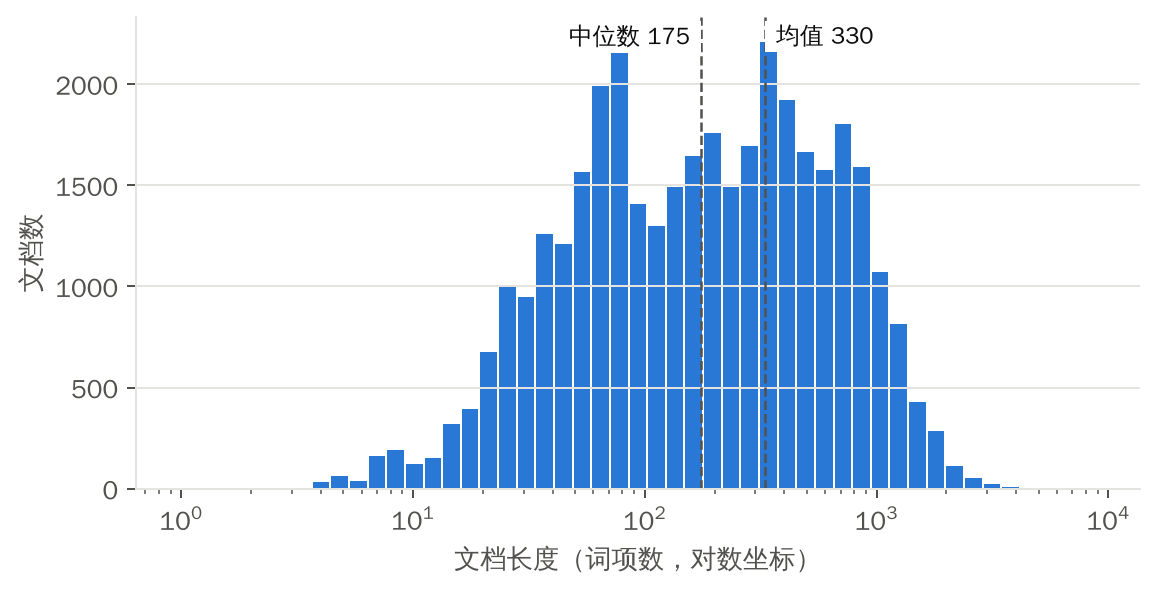
\includegraphics[width=0.85\textwidth]{figures/fig_doclen_hist.png}
\caption{TDT3 文档长度分布（不含 615 篇空文档，横轴为对数坐标）}
\label{fig:doclen}
\end{figure}

\subsection{软硬件环境}

实验运行环境如表~\ref{tab:env} 所示。搜索引擎本身只依赖 Python 标准库，没有引入任何第三方检索或自然语言处理库；matplotlib 仅用于绘制报告图表，NLTK 仅用于校验我们自行实现的 Porter 词干算法，Playwright 驱动的 Chromium 用于截取控制台输出的截图。

\begin{table}[H]
\centering
\caption{实验软硬件环境}
\label{tab:env}
\begin{tabular}{@{}lll@{}}
\toprule
类别 & 项目 & 配置 \\
\midrule
\multirow{3}{*}{硬件} & CPU & Intel Xeon Processor @ 2.10GHz，4 个逻辑核心 \\
& 内存 & 15 GiB \\
& 架构 & x86\_64 \\
\midrule
\multirow{5}{*}{软件} & 操作系统 & Ubuntu 24.04.5 LTS \\
& Python & 3.13.18（搜索引擎仅使用标准库） \\
& NLTK & 3.10.4（仅用于校验 Porter 词干实现） \\
& matplotlib & 3.11.2（报告图表） \\
& Playwright / Chromium & 1.63.0（控制台截图） \\
\midrule
编译 & XeLaTeX & TeX Live 2023/Debian，ctexart 文档类 \\
\bottomrule
\end{tabular}
\end{table}

\subsection{测试查询与观察指标}

作业指定了五条测试查询：Q1 为 \texttt{hurricane}，Q2 为 \texttt{mitch george}，Q3 为 \texttt{bill clinton israel}，Q4 为 \texttt{"newt gingrich" down}，Q5 为 \texttt{nba strike closed-door}。它们分别覆盖了单词查询、多词自由文本查询、带引号短语的混合查询和带连字符的查询。

TDT3 语料包没有附带针对这五条查询的相关性标注，因此我们无法计算准确率、召回率等基于标注的评价指标。为了让比较建立在可复现的数据上，我们为每条查询的 Top-10 结果记录了四个可直接计算的观察量：命中文档数（得分非零的文档数）、Top-10 中同时包含全部查询单元（每个查询词以及每个短语）的文档数、Top-10 文档的平均长度，以及两种模型 Top-10 结果的重合篇数。在此基础上，我们逐条阅读了 Top-10 文档的正文，对排序结果的合理性作定性判断。查询延迟取连续执行 20 次的中位数，计时范围从查询解析开始，到指定条数的结果及其摘要全部生成为止，不含索引加载时间。

\section{方法与实现}

\subsection{系统组成}

我们用 Python 实现了整个系统，代码按处理阶段划分为七个模块。\texttt{porter} 模块是依照 Porter 1980 年论文实现的词干算法；\texttt{analyzer} 模块负责分词与规范化，索引和查询共用同一个分析器，以保证两端产生的词项完全一致；\texttt{corpus} 模块读取 SGML 文件并抽取正文；\texttt{index} 模块构建、保存和加载位置倒排索引；\texttt{query} 模块把查询字符串解析为词项与短语；\texttt{scoring} 模块实现 BM25 和 TF-IDF 两种打分函数；\texttt{snippet} 模块生成查询相关摘要；命令行入口 \texttt{search.py} 把这些模块组织为一次性查询和交互式查询两种使用方式。编写的完整内容请参见随附代码。

\subsection{文本预处理}

在词干还原、大小写、数字和标点（含连字符）四个方面，我们分别决定了处理还是忽略。这些决定以“索引端和查询端对同一个词给出同一个词项”为首要原则，具体实现如清单~\ref{lst:analyzer} 所示。

\begin{lstlisting}[caption={分析器的分词正则与规范化逻辑}, label={lst:analyzer}]
_TOKEN_RE = re.compile(
    r"(?P<num>\d+(?:[.,]\d+)+)"          # 1,000  3.6  1,234.5
    r"|(?P<abbr>(?:[a-z]\.){2,})"         # u.s.  u.n.
    r"|(?P<word>[a-z0-9]+(?:['’\-][a-z0-9]+)*)"  # words, clinton's, closed-door
)

    def surface_tokens(self, text: str) -> Iterator[Tuple[List[str], int, int]]:
        """Yield (terms, start, end) for every surface token of `text`.

        `terms` has more than one element only for hyphenated words. Offsets
        refer to the original string and are used for snippet highlighting.
        """
        lowered = text.lower()
        for m in _TOKEN_RE.finditer(lowered):
            kind = m.lastgroup
            tok = m.group(kind)
            if kind == "num":
                if "." in tok and "," in tok:
                    tok = tok.replace(",", "")
                elif "," in tok:
                    tok = tok.replace(",", "")
                yield [tok], m.start(), m.end()
            elif kind == "abbr":
                yield [tok.replace(".", "")], m.start(), m.end()
            else:
                tok = tok.replace("’", "'")
                if tok.endswith("'s"):
                    tok = tok[:-2]
                tok = tok.replace("'", "")
                parts = [p for p in tok.split("-") if p]
                if parts:
                    yield [self._normalize_part(p) for p in parts], m.start(), m.end()
\end{lstlisting}

在大小写上，我们把全文统一转为小写。TDT3 的广播字幕存在大量不规范的大小写，例如同一个飓风名在 VOA 稿件中写作“Hurricane Georges”，在 NBC 字幕中写作“hurricane georges”，在 CNN 字幕中又写作“Hurricane georges”，区分大小写会把同一实体拆成多个词项，而查询词的大小写又无从约定，因此统一小写在这份语料上收益明确。

在数字上，我们选择保留数字。新闻中的年份、伤亡人数和金额本身就是有检索价值的内容，丢弃它们没有收益。为了让同一个数值只对应一个词项，我们删除了千位分隔符（“1,000”变为 \texttt{1000}），保留小数点（“3.6”保持为 \texttt{3.6}），并且不对纯数字做词干还原。

在标点上，我们删除标点，但单独处理了三类会影响词项一致性的情形。由点号连接的缩写被合并为一个词（“U.S.”变为 \texttt{us}）；英文所有格“'s”被去掉，其余撇号直接删除（“Clinton's”变为 \texttt{clinton}，“don't”变为 \texttt{dont}）；带连字符的词被拆成若干部分，并按顺序占据相邻的位置（“closed-door”变为位置相邻的 \texttt{closed} 与 \texttt{door}）。连字符拆分的意义在于，原文中写作“closed door”和“closed-door”的两种形式会得到相同的词项序列，从而都能被同一个短语查询命中。分析器为每个表层词同时返回它在原文中的字符区间，摘要模块据此定位并高亮命中词。

在词干上，我们实现并启用了 Porter 词干算法，使“hurricane”与“hurricanes”、“strike”与“strikes”、“closed”与“closing”归并为同一词项。为了确认实现的正确性，我们以 NLTK 中严格遵循原论文的 \texttt{ORIGINAL\_\allowbreak ALGORITHM} 模式作为参照，对不做词干还原的索引中的全部 110,617 个纯字母词逐一比对。两者只在 27 个词上给出不同结果，而这 27 个词的长度全部不超过两个字母（如 \texttt{us}、\texttt{is}、\texttt{as}）。差异的原因在于，我们沿用了 Porter 参考实现中“长度不超过 2 的词不做处理”的约定，而 NLTK 的原论文模式会把 \texttt{us} 还原为 \texttt{u}。除此以外，两者在全部词表上完全一致。

此外，我们决定不删除停用词。五条测试查询中的 \texttt{down} 恰好是常见的停用词表成员，删除它会使 Q4 退化为单纯的短语查询。同时，常见词的权重已经由逆文档频率自然压低（\texttt{down} 出现在 6,941 篇文档中，其 BM25 逆文档频率只有 1.69，而 \texttt{nba} 为 4.89），没有必要再通过停用词表把它们硬性剔除。不删除停用词的代价是索引中保存了 the、of 等高频词的倒排表，在本实验的规模下，这部分空间开销是可以接受的。

\subsection{位置倒排索引}

为了支持短语查询，索引必须记录每个词项在文档中的出现位置。我们为每个词项保存三个并行的无符号整数数组：\texttt{docs} 按升序记录包含该词项的文档内部编号，\texttt{tfs} 记录该词项在对应文档中的出现次数，\texttt{pos} 把所有出现位置按文档顺序首尾相接存放，第 $k$ 篇文档的位置区间可以由 \texttt{tfs} 的前缀和推出。选择 \texttt{array} 而不是嵌套的 Python 列表，是因为六百万条倒排记录若以列表存储，序列化和加载都会产生大量小对象；改用紧凑数组后，索引文件为 101.7 MiB，交互模式下加载一次只需 0.4 至 0.5 秒。构建过程如清单~\ref{lst:build} 所示。

\begin{lstlisting}[caption={索引构建的主循环}, label={lst:build}]
        for n, path in enumerate(iter_files(data_root)):
            docid, doctype, text = read_doc(path)
            d = len(idx.doc_names)
            idx.doc_names.append(docid)
            idx.doc_paths.append(os.path.relpath(path, data_root))
            idx.doc_types.append(doctype)

            local: Dict[str, List[int]] = defaultdict(list)
            for p, term in enumerate(analyzer.terms(text)):
                local[term].append(p)
            length = sum(len(v) for v in local.values())
            norm_sq = 0.0
            for term, plist in local.items():
                pst = postings[term]
                pst.docs.append(d)
                pst.tfs.append(len(plist))
                pst.pos.extend(plist)
                w = 1.0 + math.log10(len(plist))
                norm_sq += w * w
            idx.doc_len.append(length)
            idx.doc_norm.append(math.sqrt(norm_sq))
\end{lstlisting}

由于文档按编号顺序依次处理，每个词项的倒排表天然保持升序，无需额外排序。在同一趟扫描中，我们还为每篇文档预先计算了两个打分时要用到的统计量：BM25 所需的文档长度 $|d|$，以及 TF-IDF 余弦归一化所需的文档向量长度 $\lVert d \rVert$。

\subsection{查询解析与短语软匹配}

查询解析器先用正则表达式取出所有成对双引号括起的短语，其中也包括作业讲义示例所用的弯引号“ ”，再把剩余文本作为自由文本处理，如清单~\ref{lst:query} 所示。解析的结果是一组“查询单元”：单元可以是一个词项，也可以是一个短语。

\begin{lstlisting}[caption={查询解析：短语与连字符词的处理}, label={lst:query}]
    def add_group(terms, hyphenated=False):
        if not terms:
            return
        if len(terms) == 1:
            q.terms.update(terms)
            return
        mode = hyphen_mode if hyphenated else "phrase+parts"
        if mode in ("phrase+parts", "parts"):
            q.terms.update(terms)
        if mode in ("phrase", "phrase+parts"):
            q.phrases.append(tuple(terms))
            q.phrase_terms.update(terms)

    # quoted phrases first, then whatever is left is free text
    rest = []
    last = 0
    for m in _PHRASE_RE.finditer(text):
        rest.append(text[last:m.start()])
        add_group(analyzer.terms(m.group(1)))
        last = m.end()
    rest.append(text[last:])
    free = re.sub(r"[\"“”]", " ", " ".join(rest))  # unbalanced quotes
    for terms, _, _ in analyzer.surface_tokens(free):
        add_group(terms, hyphenated=True)
    return q
\end{lstlisting}

对于引号短语，我们采用“软匹配”。短语本身作为一个单元参与打分，同时短语中的每个词也作为独立单元加入查询。因此 Q4 被解析为短语单元 \texttt{(newt, gingrich)} 加上词项单元 \texttt{newt}、\texttt{gingrich} 和 \texttt{down}。包含完整短语的文档会额外获得短语单元的得分，而只零散出现这几个词的文档仍然可以被检索到，只是排名靠后。与之相对的“硬匹配”要求文档必须包含短语才能进入结果，我们把它保留为 \texttt{--strict-phrase} 选项，用于对照实验。

短语单元的文档频率和文档内频率通过位置求交得到：先从文档频率最小的词出发，求出同时包含短语中所有词的候选文档，再在每篇候选文档内检查位置 $p, p+1, \dots$ 是否依次出现短语的各个词。按这一过程统计，语料中有 409 篇文档同时含有 \texttt{newt} 和 \texttt{gingrich}，其中 406 篇含有二者相邻构成的短语。

连字符词的处理在开发中经历了一次修正。最初我们让连字符词与引号短语采用相同的规则，即短语单元加上每个组成部分。Q5 的结果暴露出这一规则的问题：\texttt{closed-door} 一个词在查询中占据了三个单元，三者的 BM25 逆文档频率之和为 11.19（短语 5.62，\texttt{close} 2.06，\texttt{door} 3.51），是 \texttt{nba} 的 4.89 的两倍多，结果排名前列的几乎都是联合国安理会“闭门磋商”的报道。用户输入的连字符词在语义上只是一个词，因此我们把默认规则改为“一个连字符词只构成一个短语单元”，原规则和“只拆成独立词项”的规则则通过 \texttt{--hyphen} 选项保留，三种规则的对照结果见第~\ref{sec:ablation} 节。

\subsection{相关性打分函数}

两种打分函数都以“单元”为单位逐个累加得分，即对每个查询单元遍历它的倒排表，把该单元对每篇文档的贡献累加到一个以文档编号为键的累加器中。下面用 $N$ 表示文档总数，$\mathrm{df}_u$ 表示包含单元 $u$ 的文档数，$\mathrm{tf}_{u,d}$ 表示单元 $u$ 在文档 $d$ 中的出现次数，$\mathrm{qtf}_u$ 表示单元 $u$ 在查询中的出现次数。

BM25 的打分公式为
\begin{gather}
\mathrm{score}(d, q) = \sum_{u \in q} \mathrm{qtf}_u \cdot \mathrm{IDF}(u) \cdot
\frac{\mathrm{tf}_{u,d}\,(k_1 + 1)}{\mathrm{tf}_{u,d} + k_1\left(1 - b + b\,\dfrac{|d|}{\mathrm{avgdl}}\right)},
\label{eq:bm25} \\
\mathrm{IDF}(u) = \ln\!\left(1 + \frac{N - \mathrm{df}_u + 0.5}{\mathrm{df}_u + 0.5}\right), \notag
\end{gather}
其中 $|d|$ 为文档长度，$\mathrm{avgdl}$ 为全体文档的平均长度，$k_1$ 控制词频饱和的速度，$b$ 控制文档长度归一化的强度。我们采用常用取值 $k_1 = 1.5$、$b = 0.75$。逆文档频率中的“$1+$”保证了即使某个词出现在过半文档中，它的权重也不会变为负数，这对于不删除停用词的系统是必要的。由公式~\eqref{eq:bm25} 可知，当 $\mathrm{tf}_{u,d}$ 趋于无穷时，单个单元的贡献上限为 $\mathrm{IDF}(u)\,(k_1+1)$。对于 Q1 的 \texttt{hurricane}，这一上限为 $4.022 \times 2.5 = 10.06$。清单~\ref{lst:bm25} 是对应实现，其中长度归一化因子对每篇文档只计算一次并缓存。

\begin{lstlisting}[caption={BM25 打分}, label={lst:bm25}]
    def score(self, index, query, restrict=None):
        N = index.num_docs
        K = self._length_norm(index)
        k1p1 = self.k1 + 1
        acc = defaultdict(float)
        for unit, qw, docs, tfs in _units(index, query, self.phrase_weight):
            df = len(docs)
            w = qw * math.log(1 + (N - df + 0.5) / (df + 0.5))
            for d, tf in zip(docs, tfs):
                if restrict is None or d in restrict:
                    acc[d] += w * tf * k1p1 / (tf + K[d])
        return acc
\end{lstlisting}

TF-IDF 向量空间模型采用 SMART 记法中的 lnc.ltc 方案。查询向量中单元 $u$ 的权重为 $w_{q,u} = (1 + \log_{10}\mathrm{qtf}_u)\cdot\log_{10}(N/\mathrm{df}_u)$，随后做余弦归一化；文档向量中的权重为对数词频除以文档向量长度：
\begin{equation}
w_{d,u} = \frac{1 + \log_{10}\mathrm{tf}_{u,d}}{\lVert d \rVert},
\qquad
\lVert d \rVert = \sqrt{\sum_{t \in d} \left(1 + \log_{10}\mathrm{tf}_{t,d}\right)^2},
\qquad
\mathrm{score}(d, q) = \sum_{u \in q} \frac{w_{q,u}}{\lVert q \rVert}\, w_{d,u}.
\label{eq:tfidf}
\end{equation}
文档向量长度 $\lVert d \rVert$ 在建索引时对文档的全部词项求和得到。短语单元没有计入 $\lVert d \rVert$，因为短语只在查询时才会被构造出来，所以当查询含短语时，得分不再严格限定在 $[0, 1]$ 之内，但这不影响同一查询内的排序。实现如清单~\ref{lst:tfidf} 所示。

\begin{lstlisting}[caption={TF-IDF（lnc.ltc）打分}, label={lst:tfidf}]
    def score(self, index, query, restrict=None):
        N = index.num_docs
        norms = index.doc_norm
        units = list(_units(index, query, self.phrase_weight))
        wq = []
        for unit, qw, docs, tfs in units:
            idf = math.log10(N / len(docs))
            wq.append((1 + math.log10(qw)) * idf if qw >= 1 else qw * idf)
        qnorm = math.sqrt(sum(w * w for w in wq)) or 1.0
        acc = defaultdict(float)
        for (unit, qw, docs, tfs), w in zip(units, wq):
            w /= qnorm
            if w == 0.0:
                continue
            for d, tf in zip(docs, tfs):
                if restrict is None or d in restrict:
                    acc[d] += w * (1 + math.log10(tf)) / norms[d]
        return acc
\end{lstlisting}

累加结束后，我们用堆选出得分最高的若干篇文档，篇数由 \texttt{--hits} 指定。得分相同时按文档内部编号排序，以保证同一查询的输出完全确定、可以复现。

\subsection{摘要生成与命令行交互}

摘要模块为每篇结果文档挑选一个包含 36 个连续表层词的窗口。选择窗口的依据依次为：窗口内出现的不同查询词数量越多越好；其次优先包含完整短语的窗口；再次是命中词的总次数更多；以上都相同时取最靠前的窗口。窗口向左多保留三个词作为上下文，正文中的硬换行被压缩为空格，窗口不在文档首尾时用省略号标示。在终端中，命中的查询词以黄色粗体高亮，文档编号以青色显示；当输出被重定向到文件时，程序自动关闭颜色，输出纯文本。

命令行入口支持两种用法。一次性查询直接把查询词写在命令后面，例如 \texttt{./search --hits=27 new york san francisco}，其中 \texttt{--hits} 指定返回条数，\texttt{--model} 在 \texttt{bm25} 与 \texttt{tfidf} 之间切换。由于 shell 会剥去参数中的双引号，带短语的查询在一次性模式下需要写成 \texttt{'"newt gingrich"' down}。为了让短语查询能按作业示例的写法直接输入，我们另外实现了交互模式：不带查询词启动程序后，加载一次索引，随后在提示符“\#”后输入 \texttt{search --hits=10 "newt gingrich" down} 这样的命令即可。交互模式逐条为查询编号，输出格式为“\texttt{q1 = 查询 (took 秒数 seconds)}”，与作业给出的参考格式保持一致。

\section{实验结果}

\subsection{索引构建}

表~\ref{tab:index} 汇总了两套索引的规模：一套启用 Porter 词干还原，作为系统默认配置；另一套不做词干还原，用于消融对照。

\begin{table}[H]
\centering
\caption{索引规模与构建开销}
\label{tab:index}
\begin{tabular}{@{}lrr@{}}
\toprule
指标 & 启用词干还原 & 不做词干还原 \\
\midrule
文档数 & 37,526 & 37,526 \\
词项总数（全部位置） & 12,389,223 & 12,389,223 \\
词表大小 & 92,128 & 122,340 \\
只出现一次的词项数 & 34,598 & 43,006 \\
倒排记录数（词项--文档对） & 6,006,714 & 6,361,761 \\
索引文件大小 & 101.7 MiB & 106.4 MiB \\
构建时间 & 约 22 秒 & 约 22 秒 \\
\bottomrule
\end{tabular}
\end{table}

词干还原把词表从 122,340 个词项压缩到 92,128 个，减少了 24.7\%；倒排记录数只减少了 5.6\%。两者差距悬殊的原因在于，被归并的大多是同一个词的屈折变形，例如“hurricane”与“hurricanes”，而这些变形往往同时出现在同一篇文档中。归并之后，它们在这篇文档里只留下一条倒排记录，因此减少的记录数远少于减少的词表项。位置信息的总量与是否做词干还原无关，两套索引都保存了 1,238 万个位置，这部分构成了索引文件的主体，所以两套索引的文件大小只相差 4.7 MiB。

\subsection{五条测试查询的 BM25 检索结果}

图~\ref{fig:q1} 至图~\ref{fig:q5} 是系统默认配置（BM25，$k_1 = 1.5$，$b = 0.75$，启用词干还原）下五条测试查询的 Top-10 控制台截图。截图中的命令都是在交互模式的提示符后输入的。表~\ref{tab:queries} 汇总了这五条查询在两种打分函数下的观察量。

\begin{figure}[H]
\centering
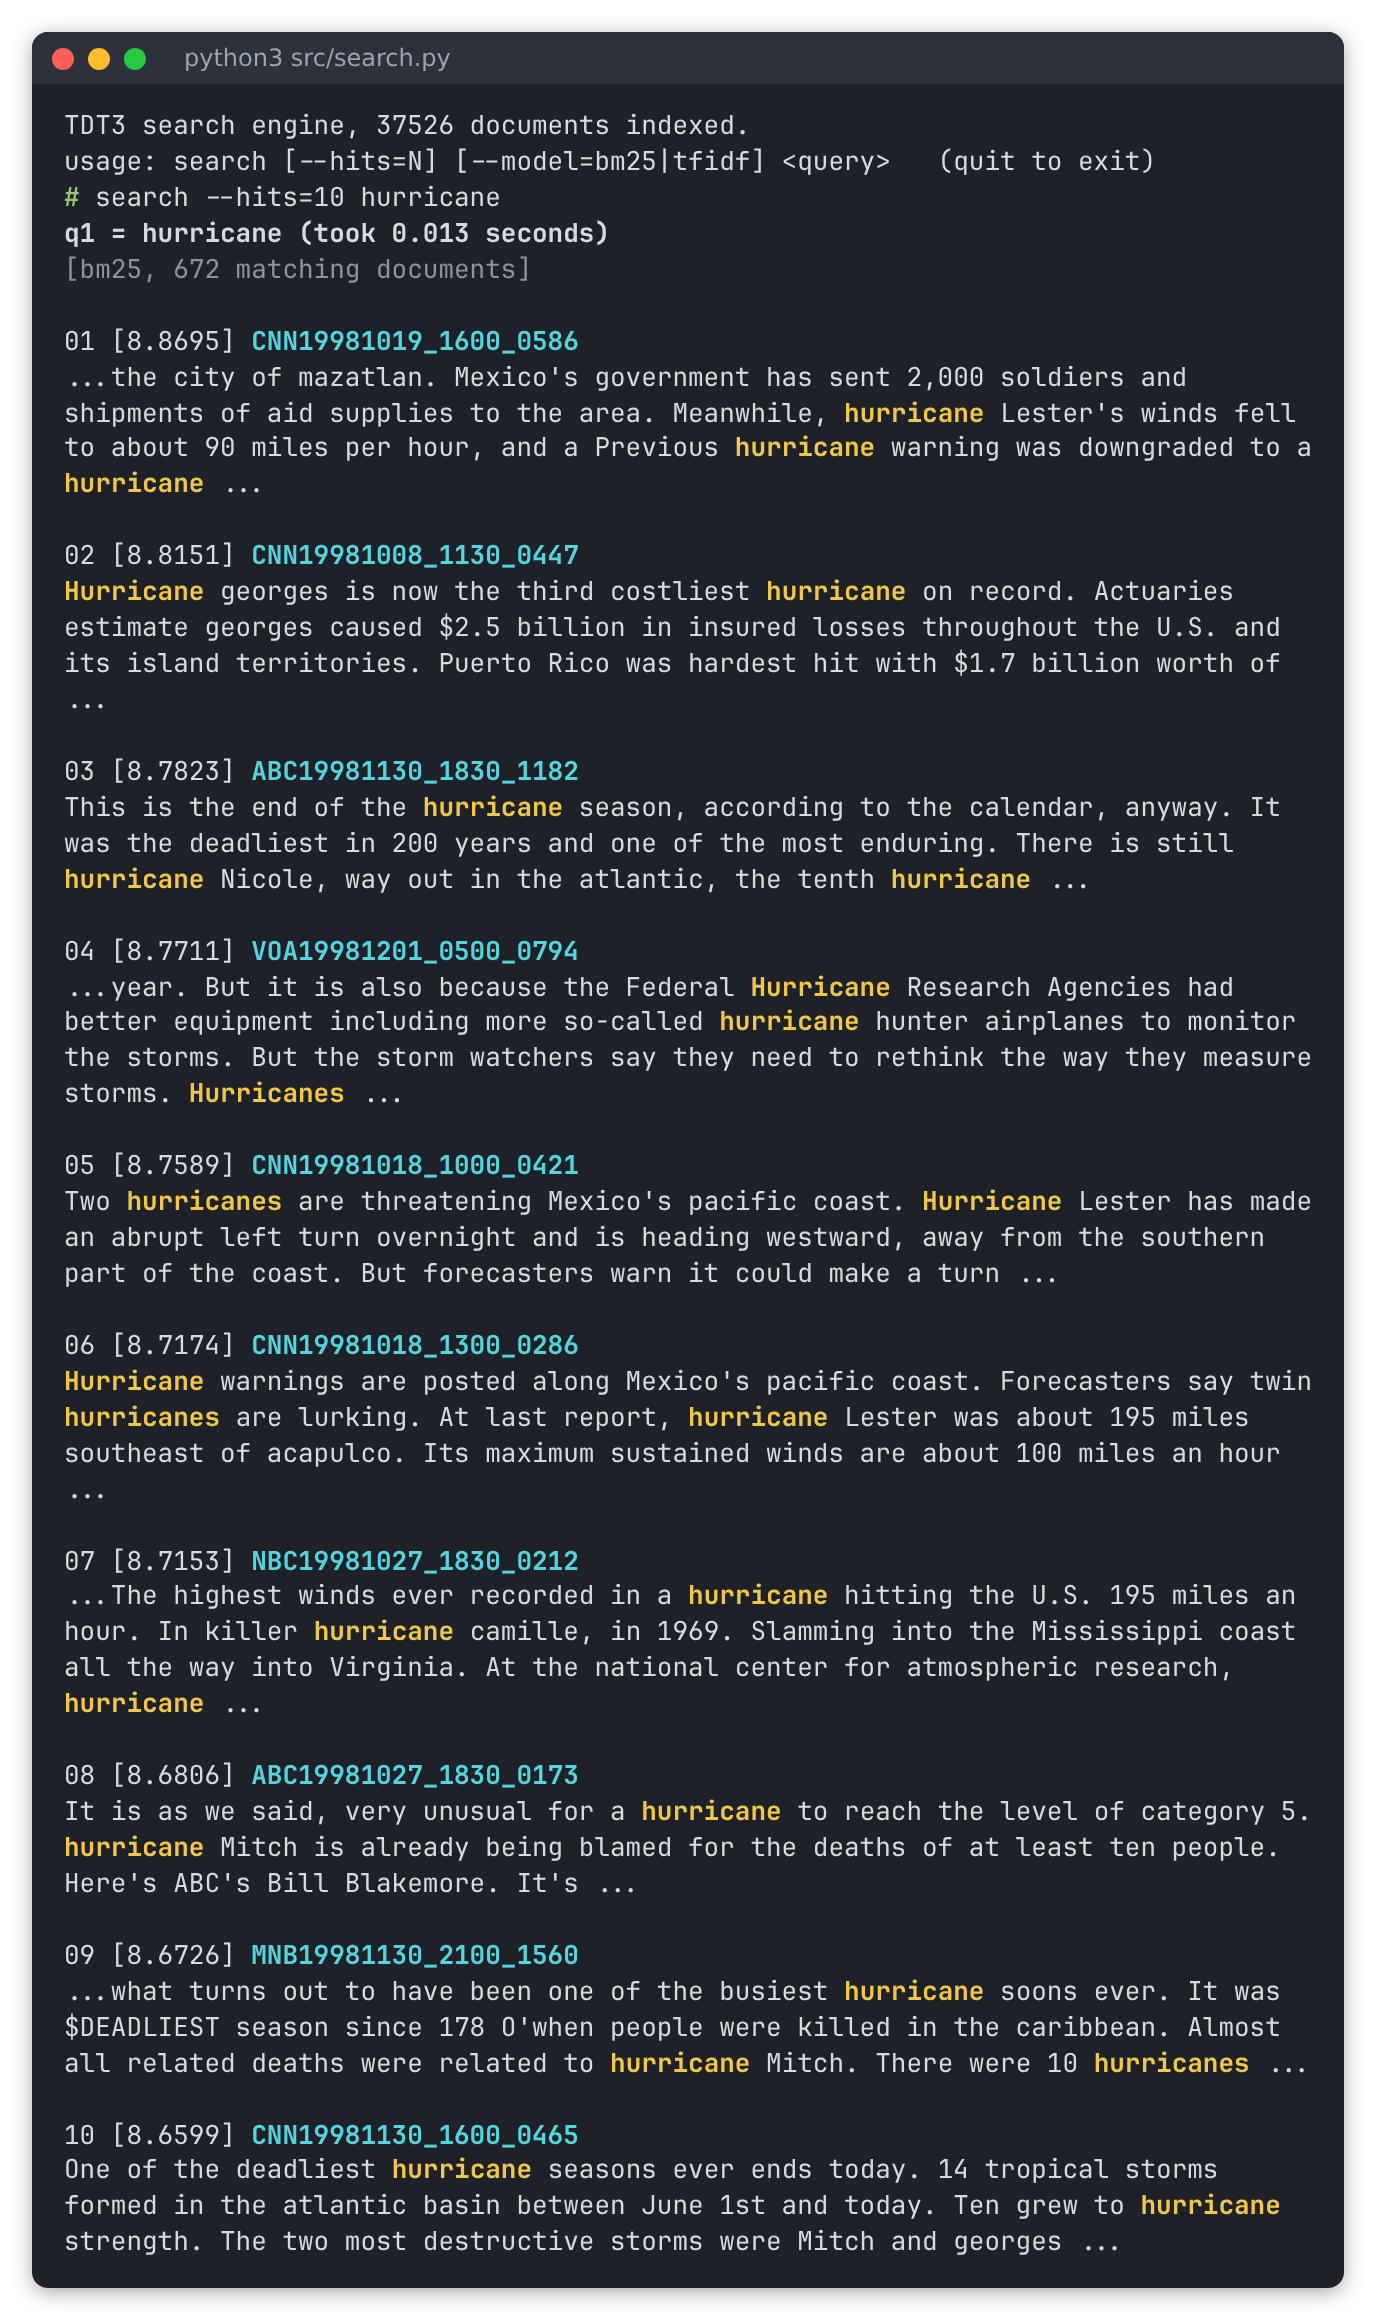
\includegraphics[width=0.78\textwidth]{figures/screen_q1_bm25.png}
\caption{Q1 \texttt{hurricane} 的 BM25 Top-10 结果}
\label{fig:q1}
\end{figure}

Q1 只有一个词，命中 672 篇文档。Top-10 全部是关于飓风的报道，内容涉及 Lester、Georges、Mitch、Nicole 等飓风，以及 1998 年飓风季的总结。十篇文档的得分集中在 8.66 至 8.87 之间，都已逼近单词查询的得分上限 10.06，说明在词频饱和之后，排序主要由文档长度决定：排名第 1 的文档长 86 个词项，“hurricane”出现了 5 次；排名第 4 的 VOA 报道长 577 个词项，出现了 16 次，较高的词频补偿了它的长度惩罚。

\begin{figure}[H]
\centering
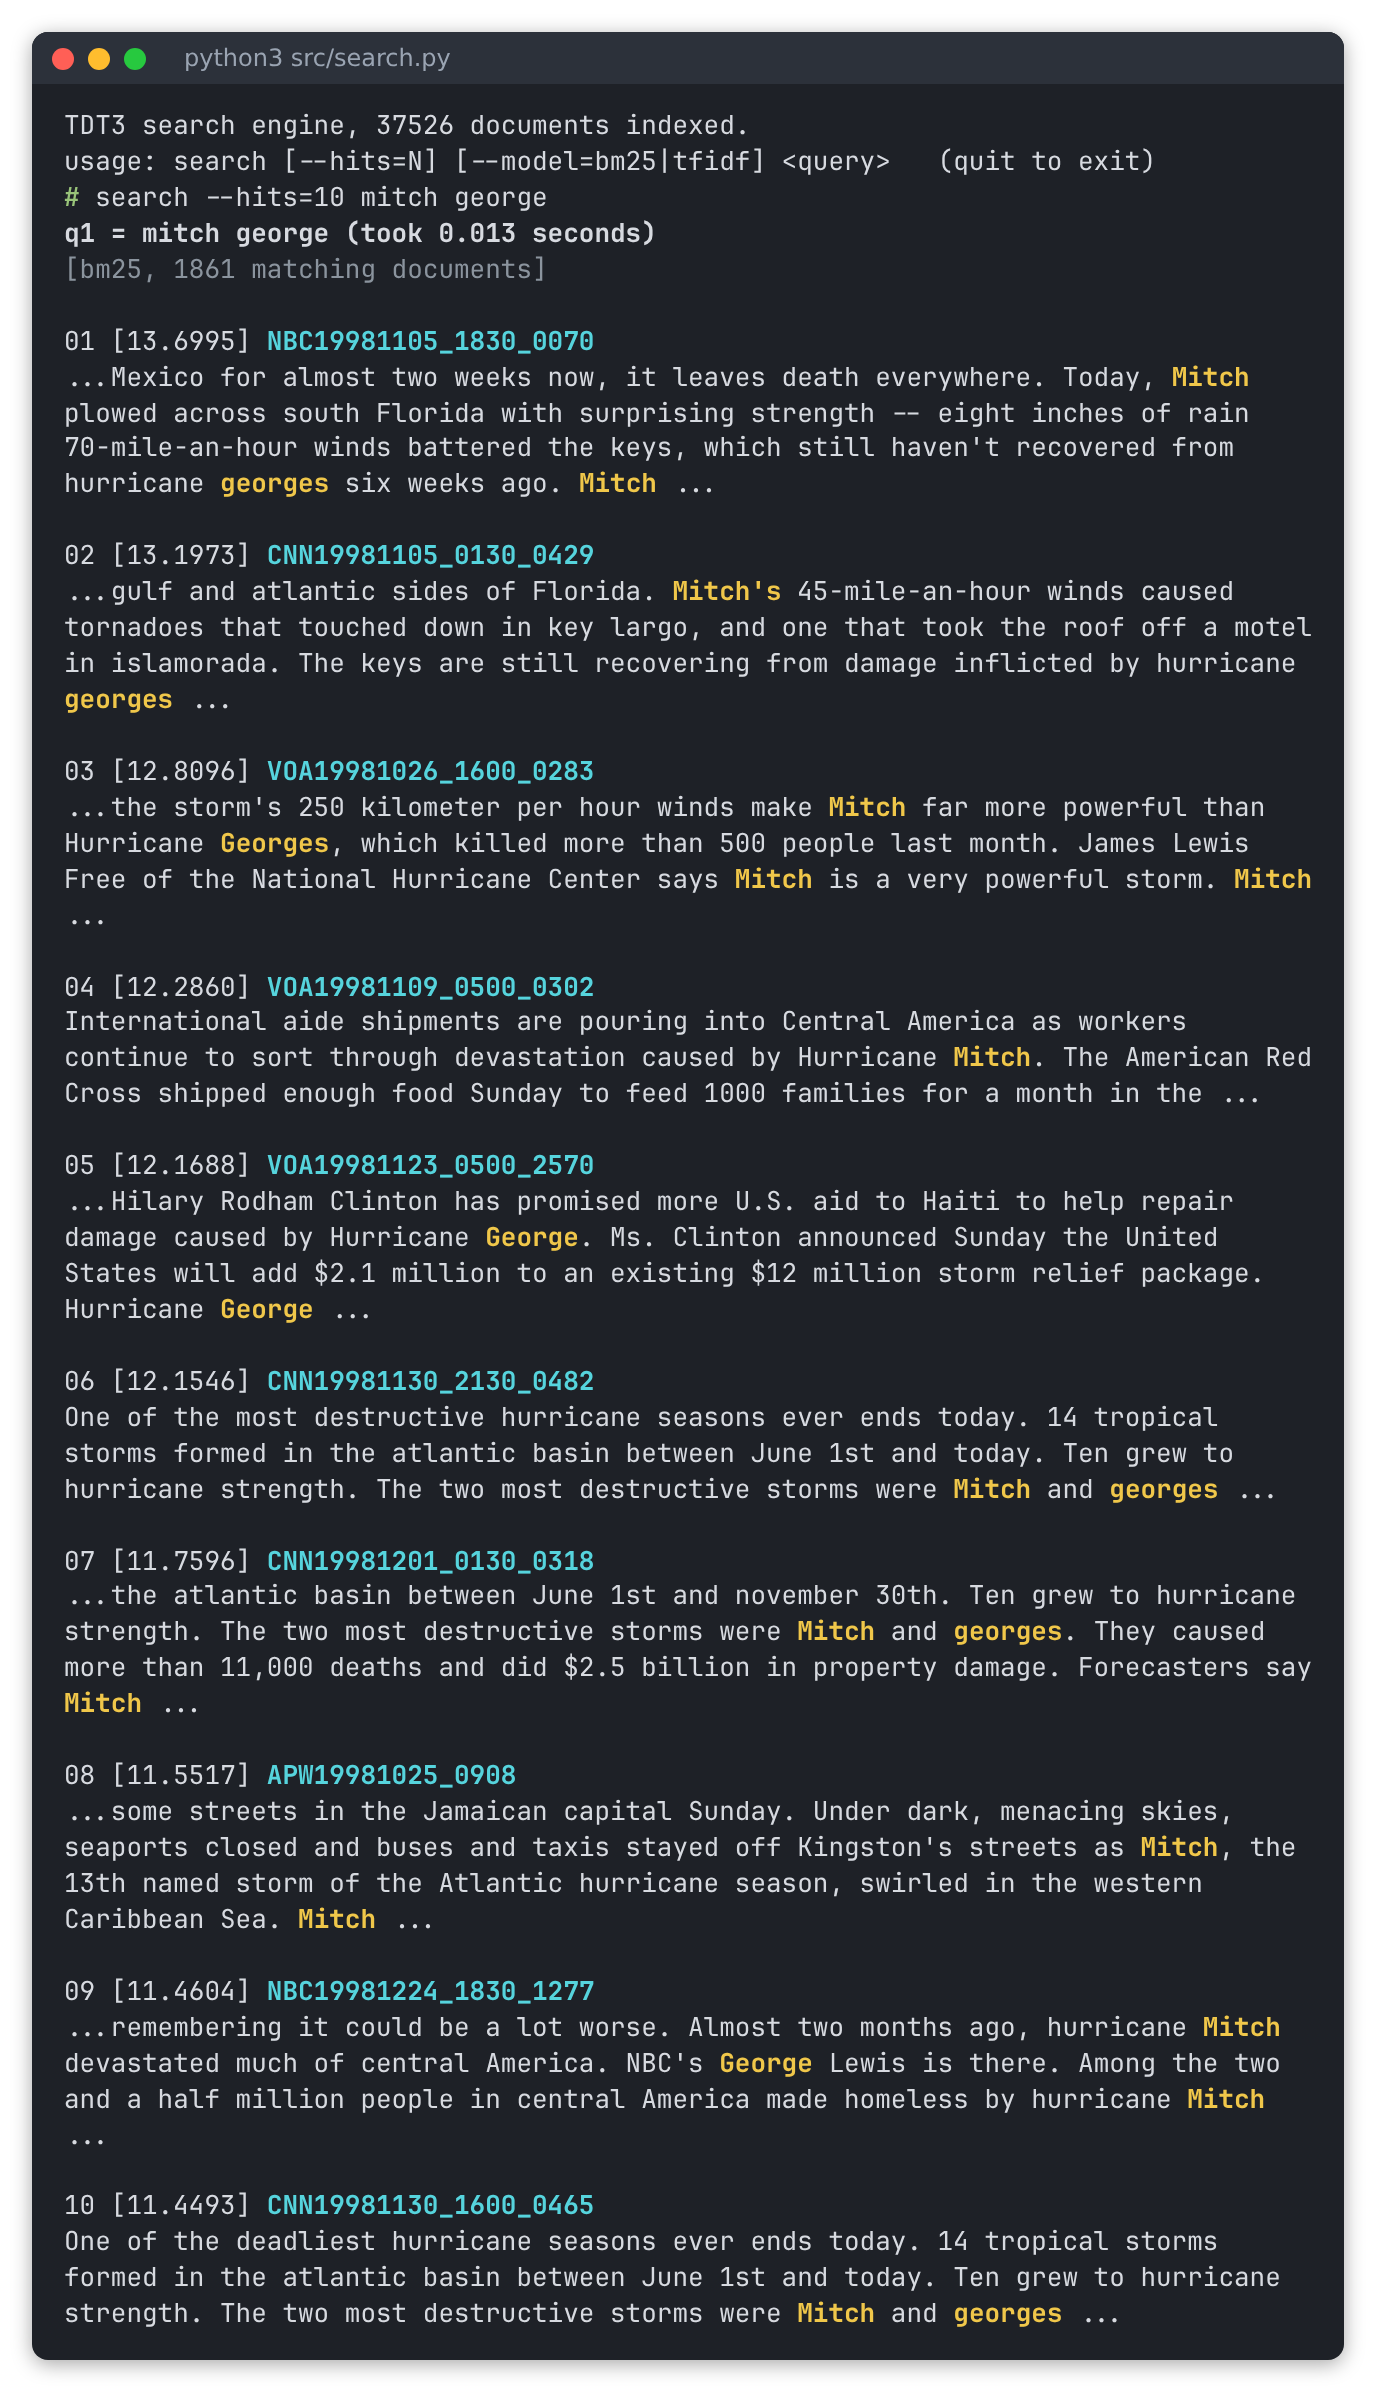
\includegraphics[width=0.78\textwidth]{figures/screen_q2_bm25.png}
\caption{Q2 \texttt{mitch george} 的 BM25 Top-10 结果}
\label{fig:q2}
\end{figure}

Q2 的十篇结果都同时含有 \texttt{mitch} 与 \texttt{georg} 两个词项，内容几乎都是同时提到飓风 Mitch 与飓风 Georges 的报道。这一结果得益于词干还原：“georges”被 Porter 算法还原为 \texttt{georg}，与查询词“george”的还原结果相同，查询由此自然覆盖了飓风 Georges 的名字。其中排名第 5 的 VOA 文档把飓风名拼写成了“Hurricane George”，也被正确召回。排名第 9 的 NBC 文档则属于名字巧合：它在报道飓风 Mitch 的同时提到了记者“George Lewis”。

\begin{figure}[H]
\centering
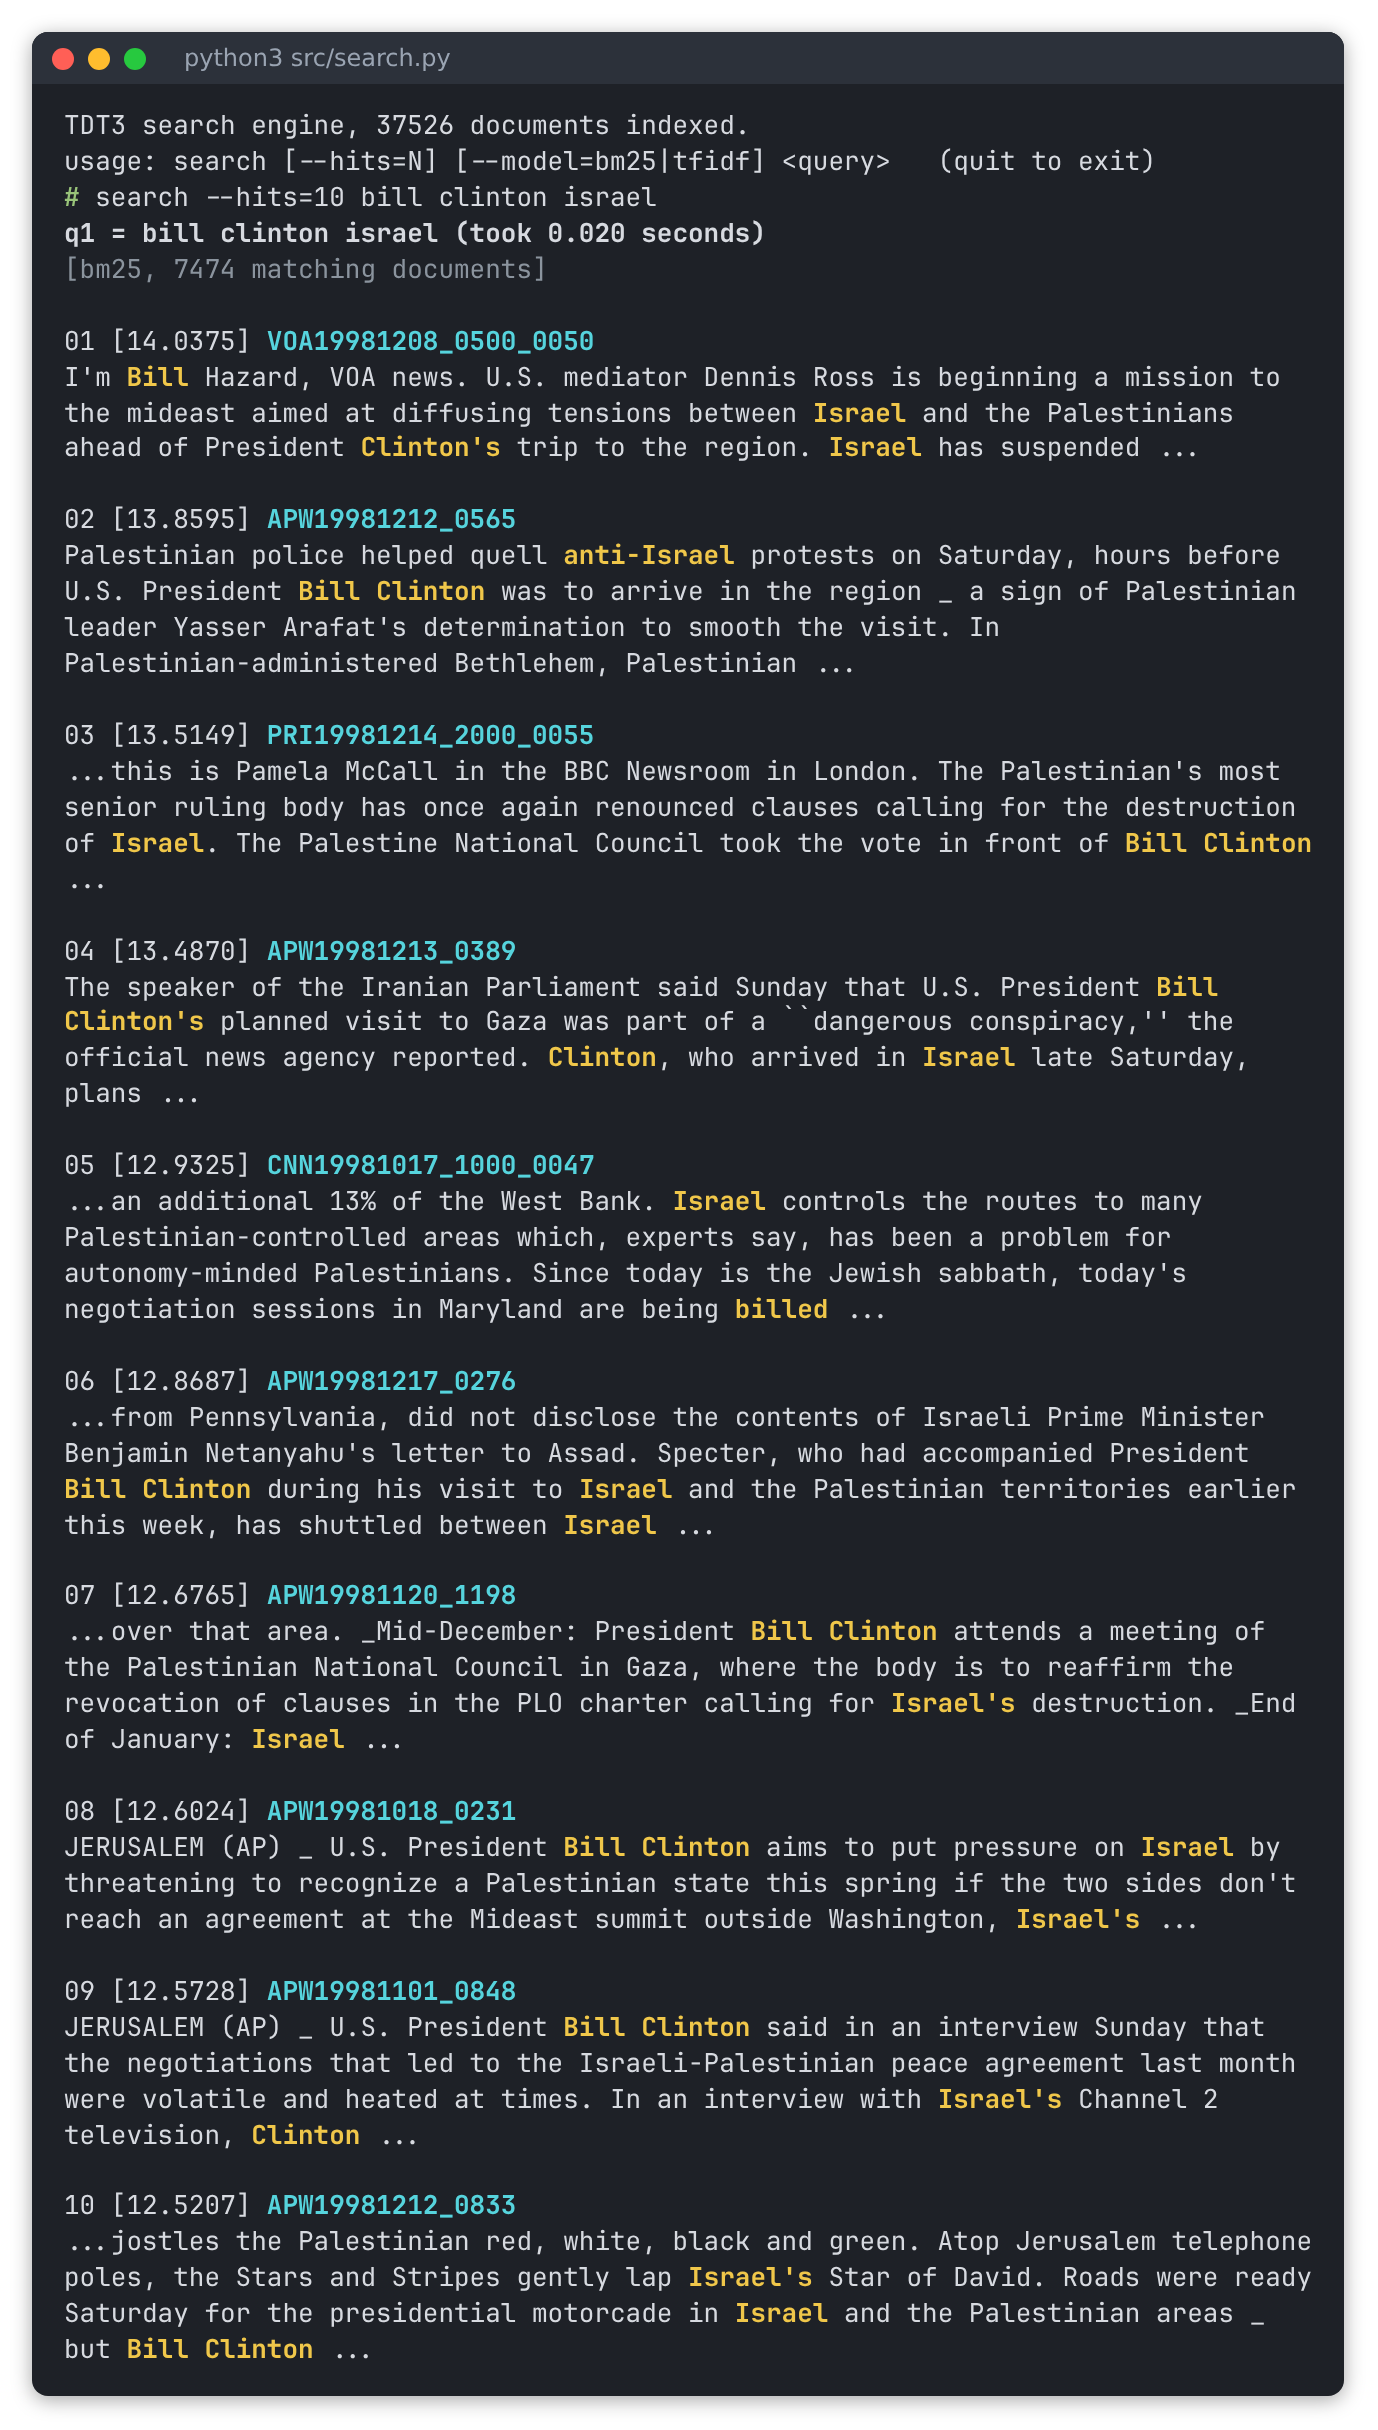
\includegraphics[width=0.78\textwidth]{figures/screen_q3_bm25.png}
\caption{Q3 \texttt{bill clinton israel} 的 BM25 Top-10 结果}
\label{fig:q3}
\end{figure}

Q3 命中 7,474 篇文档。Top-10 全部同时包含三个查询词，其中七篇来自美联社，集中报道 1998 年 12 月克林顿访问以色列和加沙、怀伊河协议后续进展等事件。结果中也出现了词干还原和一词多义带来的偏差：排名第 1 的 VOA 文档以“I'm Bill Hazard, VOA news”开头，这里的“Bill”是记者的名字；排名第 5 的 CNN 文档命中的是“being billed”，经词干还原后与查询词 \texttt{bill} 相同。这两篇文档的主体仍然是以色列与巴勒斯坦的谈判，与查询意图相符，但它们排名靠前的部分原因来自错误的词项匹配。

\begin{figure}[H]
\centering
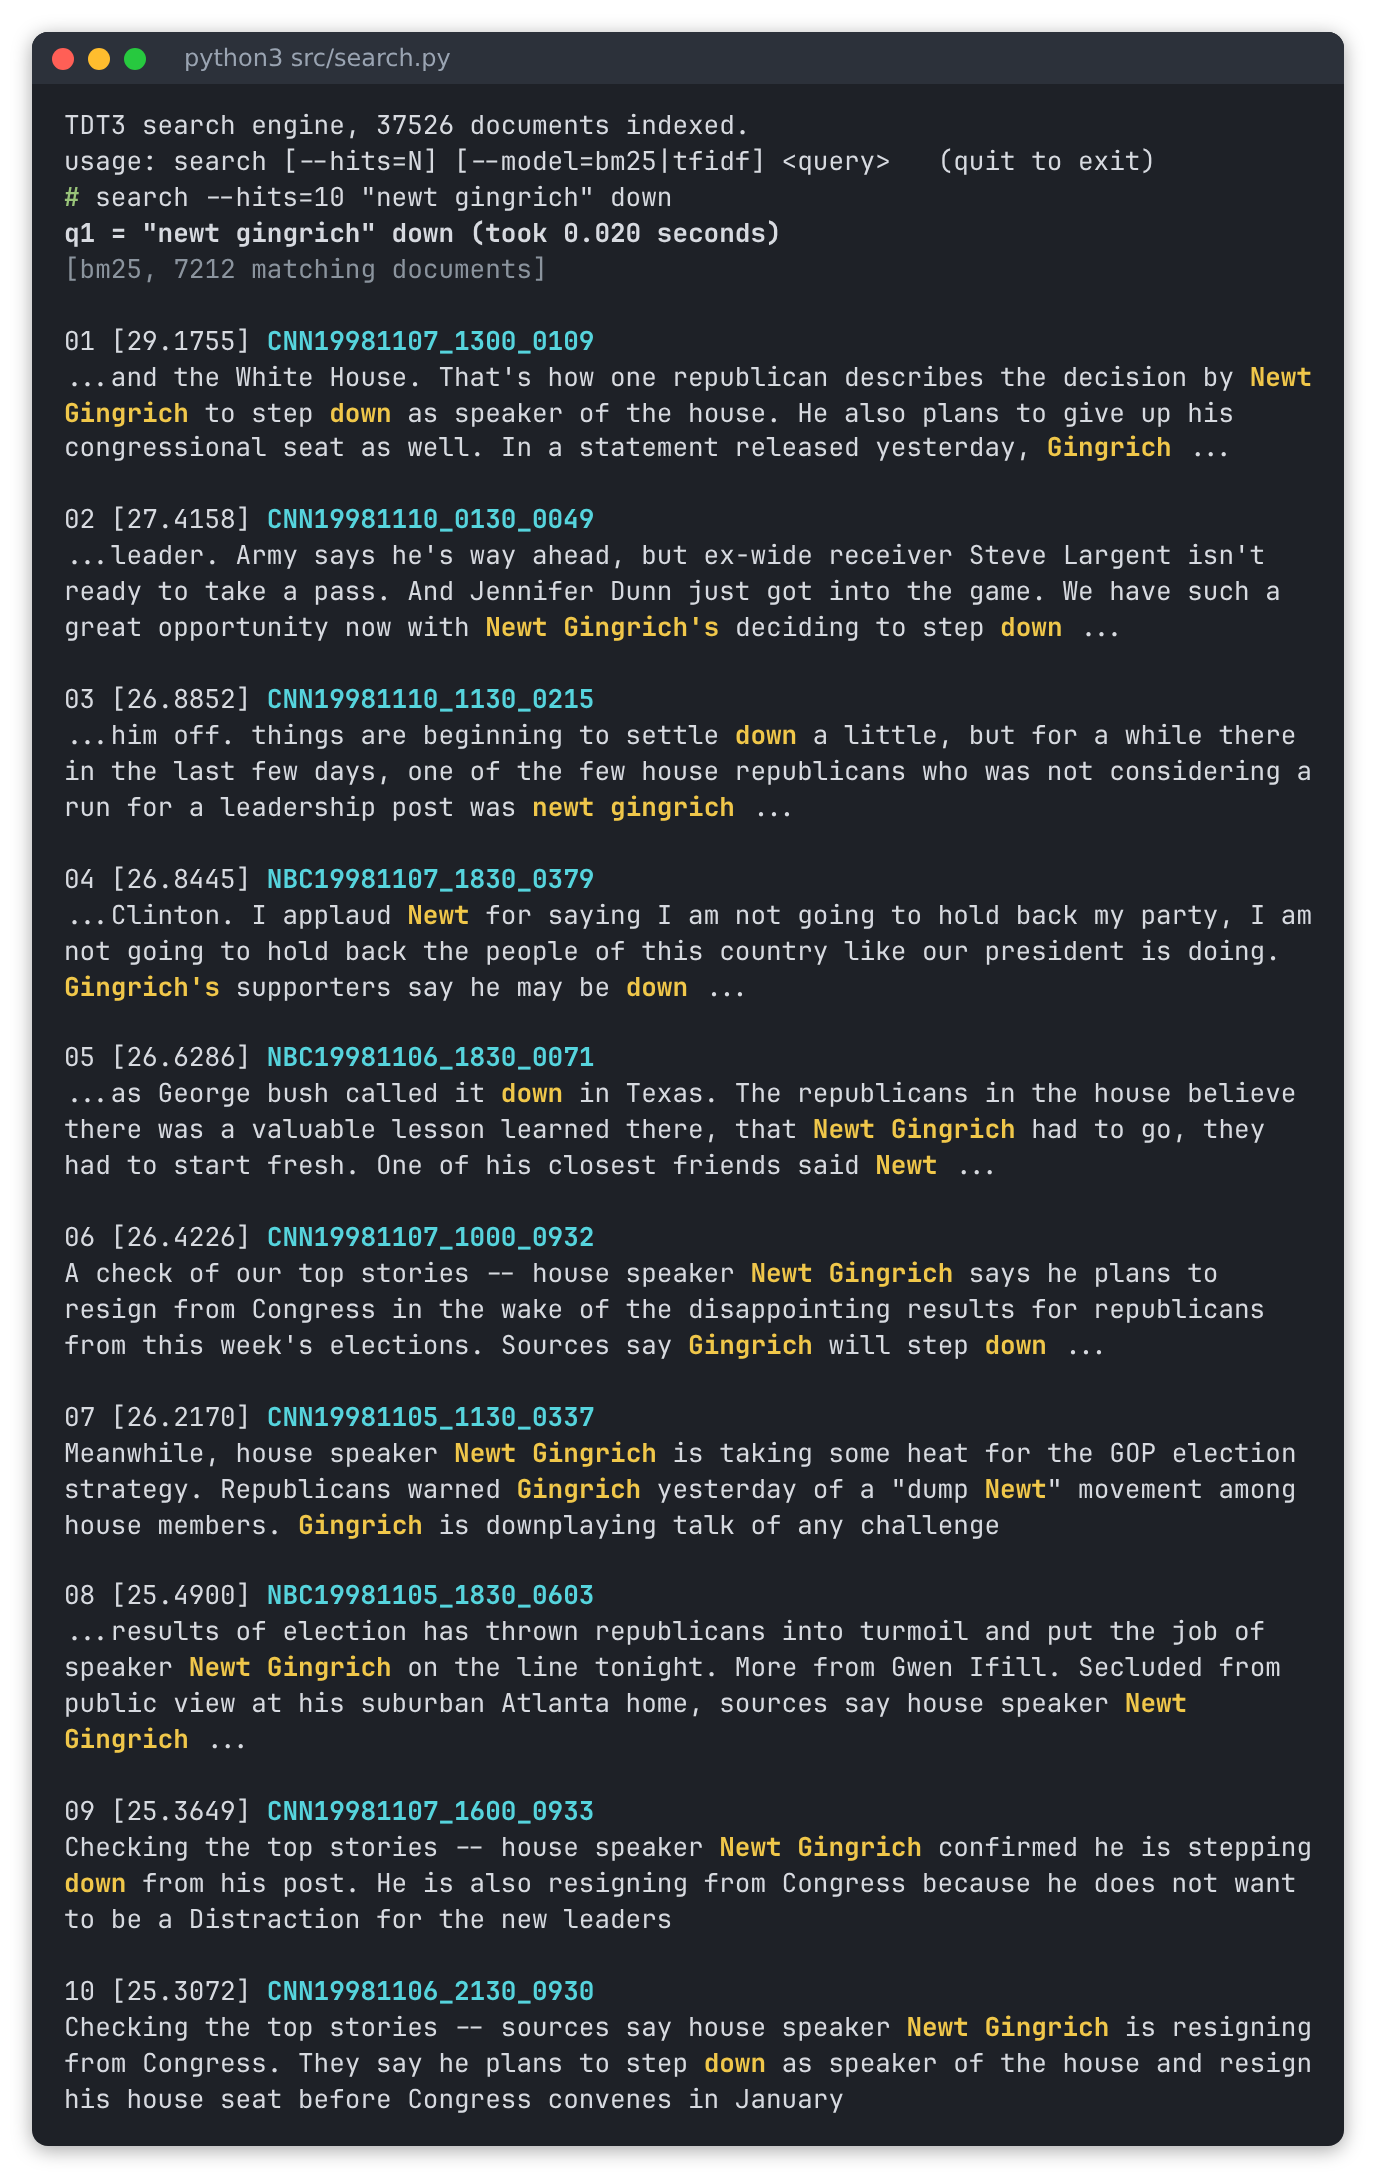
\includegraphics[width=0.78\textwidth]{figures/screen_q4_bm25.png}
\caption{Q4 \texttt{"newt gingrich" down} 的 BM25 Top-10 结果}
\label{fig:q4}
\end{figure}

Q4 的十篇结果全部包含完整短语“newt gingrich”，其中九篇同时含有 \texttt{down}，内容集中在 1998 年 11 月金里奇宣布辞去众议院议长一职（step down）的报道上。第 1 名得分 29.18，明显高于 Q1 至 Q3 的最高分，原因是短语单元与两个组成词各自贡献了一份得分，这正是软匹配所设计的“命中短语则大幅加分”的效果。

\begin{figure}[H]
\centering
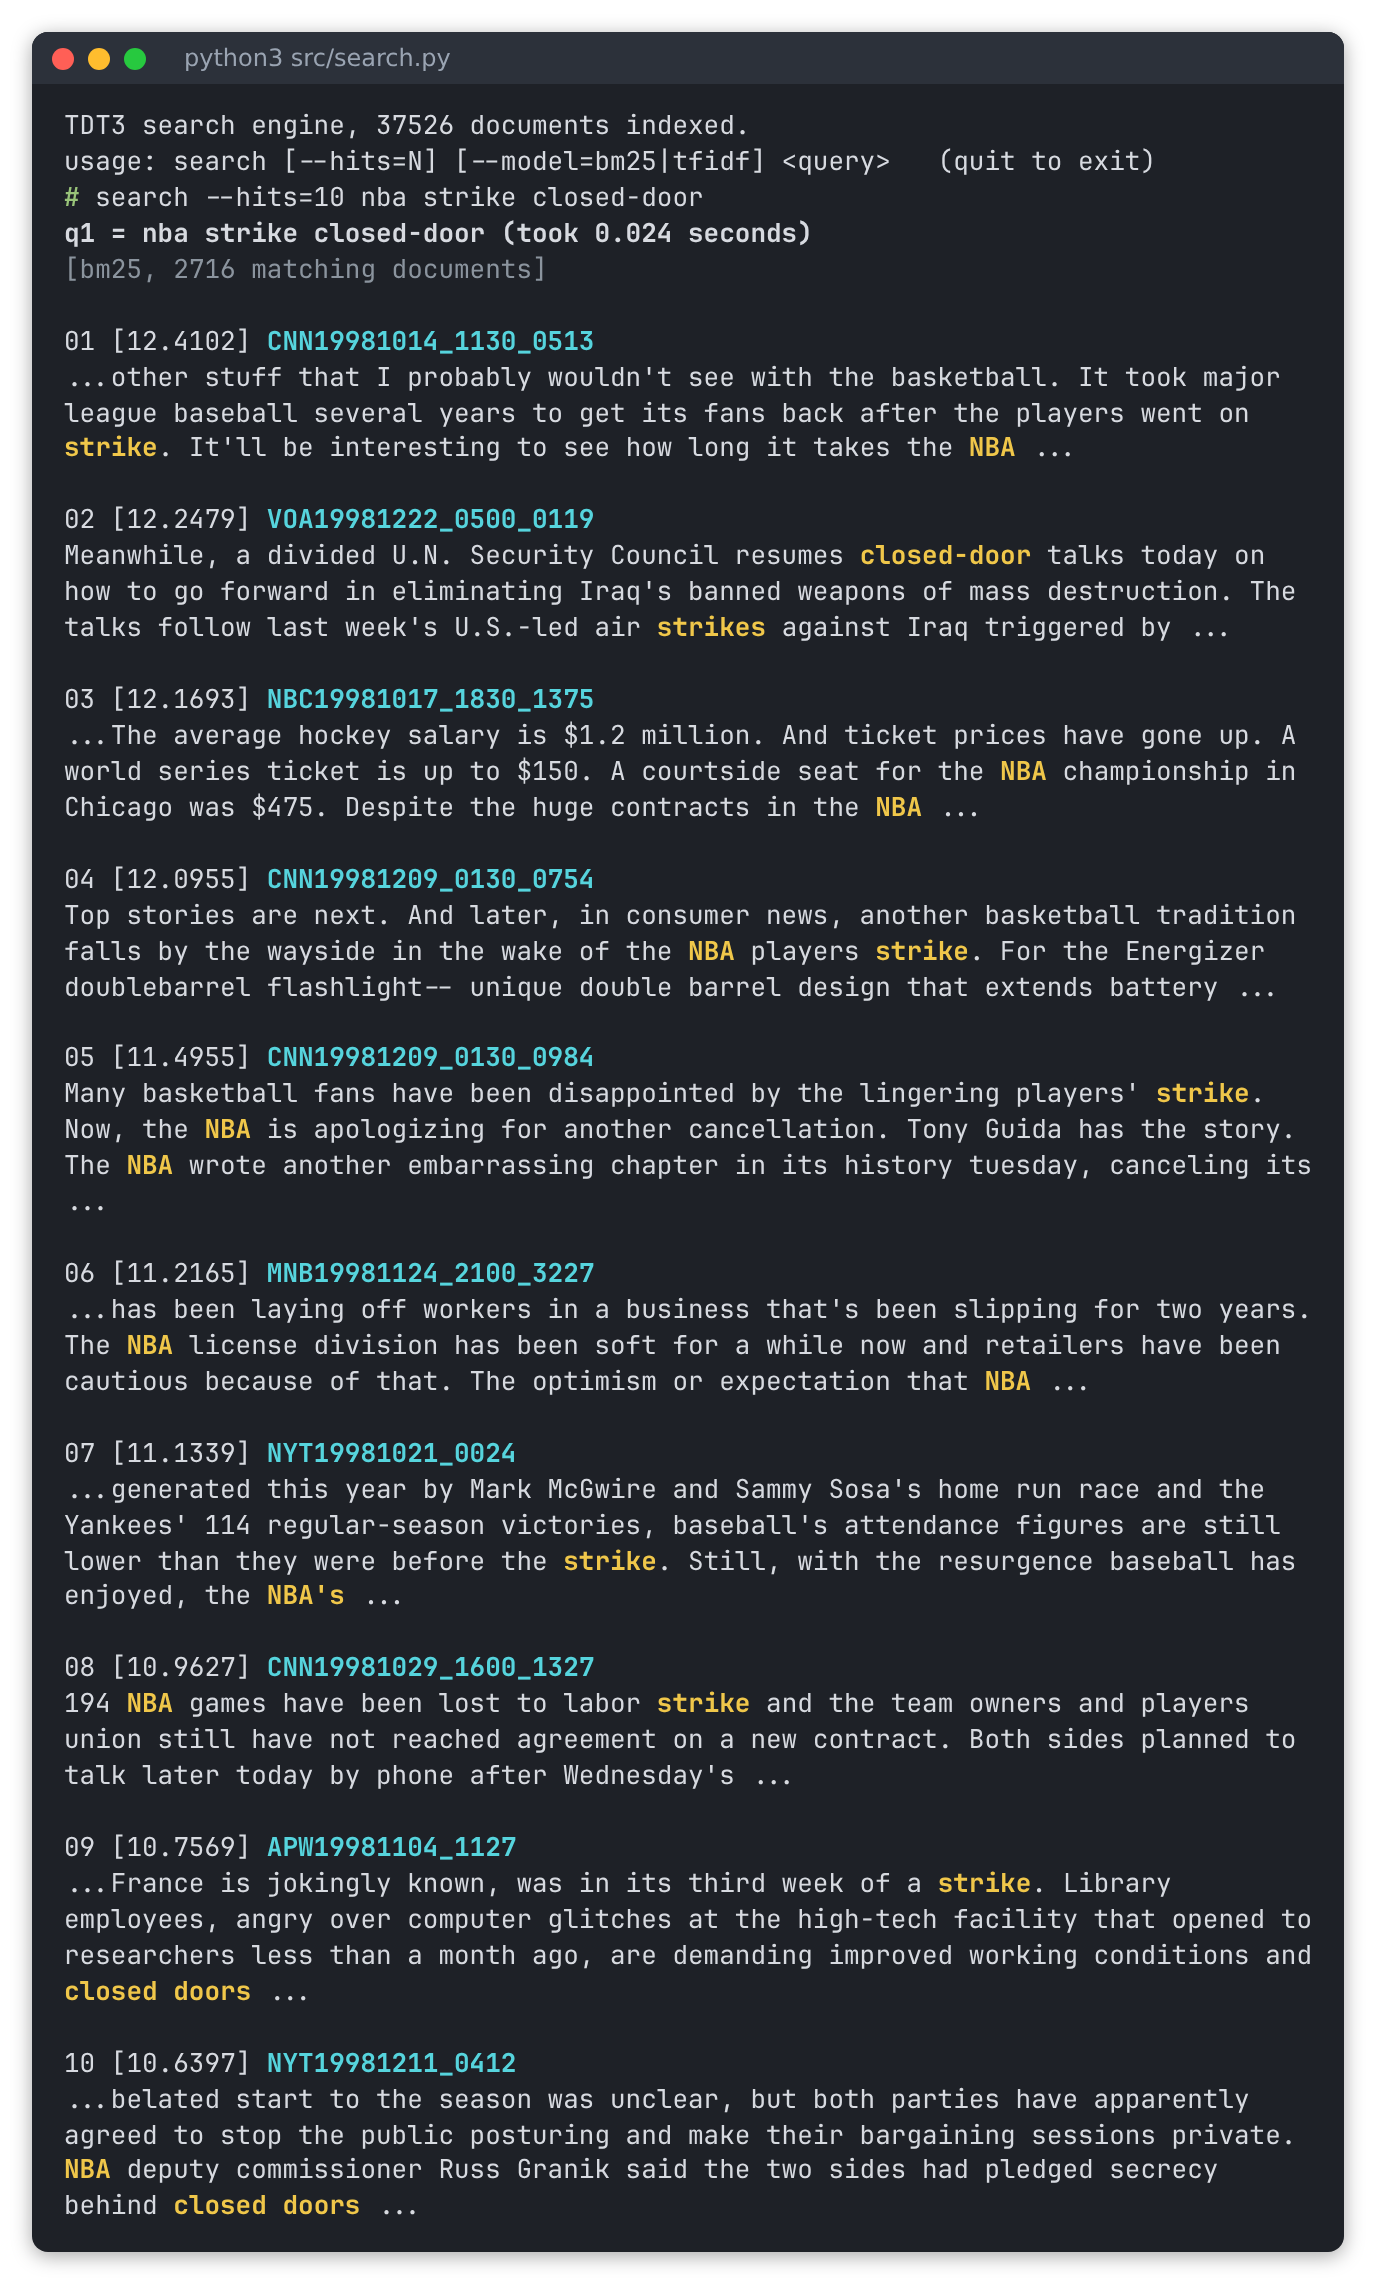
\includegraphics[width=0.78\textwidth]{figures/screen_q5_bm25.png}
\caption{Q5 \texttt{nba strike closed-door} 的 BM25 Top-10 结果}
\label{fig:q5}
\end{figure}

Q5 的 Top-10 中有八篇与 NBA 停摆有关，另外两篇分别是联合国安理会的闭门磋商（第 2 名）和埃菲尔铁塔员工罢工（第 9 名）。只有第 10 名的 NYT 文档同时包含三个查询单元，原文写道 NBA 劳资双方“pledged secrecy behind closed doors”。全语料中同时含有 \texttt{nba} 和短语 \texttt{closed door} 的文档只有 2 篇，同时含有三个查询单元的只有这 1 篇，所以 Top-10 中“全部单元命中”的文档数为 1，已经达到了语料所能提供的上限。

\begin{table}[H]
\centering
\caption{五条测试查询的观察量（Top-10，延迟为 20 次执行的中位数）}
\label{tab:queries}
\resizebox{\textwidth}{!}{\begin{tabular}{@{}l r rrrr rrrr r@{}}
\toprule
& & \multicolumn{4}{c}{BM25} & \multicolumn{4}{c}{TF-IDF（lnc.ltc）} & \\
\cmidrule(lr){3-6}\cmidrule(lr){7-10}
查询 & 命中数 & 全命中 & 平均长度 & 延迟 & 无摘要 & 全命中 & 平均长度 & 延迟 & 无摘要 & 重合 \\
\midrule
Q1 & 672   & 10 & 180.5 & 3.8  & 0.15 & 10 & 29.4 & 0.7 & 0.16 & 1 \\
Q2 & 1,861 & 10 & 168.9 & 4.0  & 0.44 & 3  & 37.3 & 1.2 & 0.44 & 3 \\
Q3 & 7,474 & 10 & 277.1 & 8.1  & 2.01 & 3  & 64.0 & 3.4 & 2.02 & 3 \\
Q4 & 7,212 & 9  & 262.1 & 8.5  & 2.83 & 0  & 23.7 & 3.7 & 2.97 & 1 \\
Q5 & 2,716 & 1  & 389.6 & 13.8 & 2.66 & 0  & 17.8 & 3.2 & 2.64 & 0 \\
\bottomrule
\end{tabular}}

\vspace{0.4em}
\parbox{0.95\textwidth}{\footnotesize “全命中”为 Top-10 中包含全部查询单元的文档数；“平均长度”以词项计，语料平均为 330.2；延迟单位为毫秒，“无摘要”列为不生成摘要时的延迟；“重合”为两种模型 Top-10 的共同文档数。两种模型的命中数相同，因为二者都对至少包含一个查询单元的文档打分。}
\end{table}

五条查询的延迟都在 14 毫秒以内。去掉摘要生成后，延迟降到 0.15 至 3 毫秒，说明一次查询的大部分时间花在读取十篇结果文档并扫描摘要窗口上，打分本身的开销很小。

\subsection{BM25 与 TF-IDF 的排序对比}

两种打分函数在同一索引上给出的结果差别很大：五条查询的 Top-10 平均只有 1.6 篇重合，Q5 甚至一篇也不重合。TF-IDF 的五组 Top-10 截图见附录~\ref{app:tfidf}。图~\ref{fig:top10len} 把两种模型返回的每篇文档的长度画在同一坐标中，差异的方向一目了然：BM25 的 Top-10 平均长度在 169 至 390 个词项之间，接近语料平均值 330.2；TF-IDF 的 Top-10 平均长度只有 18 至 64 个词项，五条查询的 Top-10 文档没有一篇超过 150 个词项。

\begin{figure}[H]
\centering
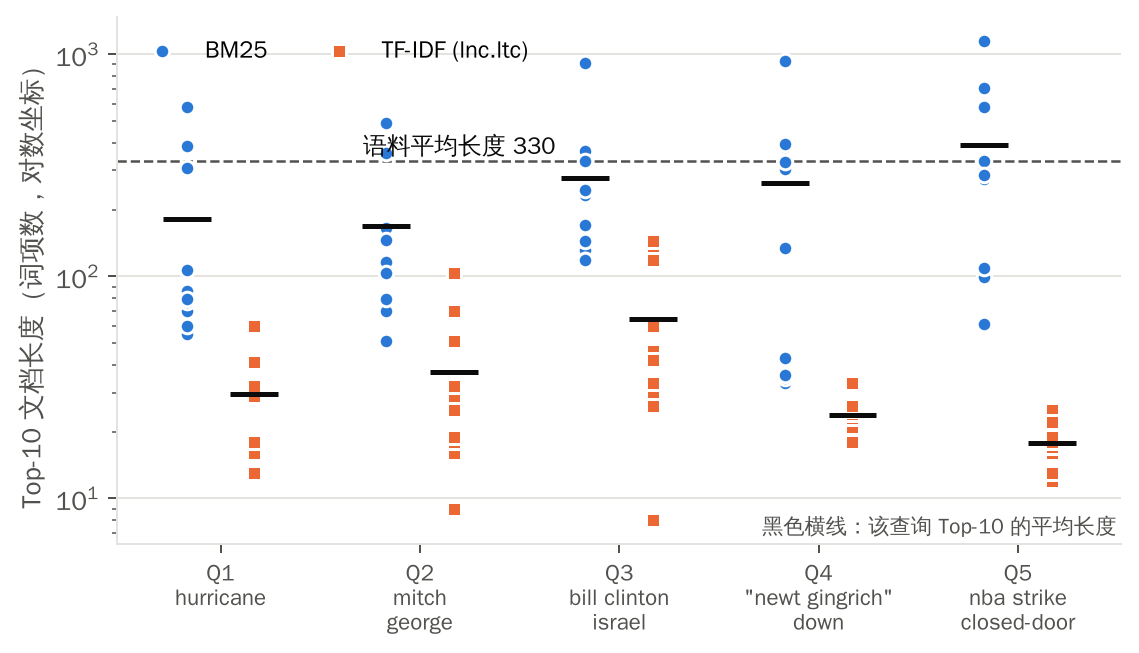
\includegraphics[width=0.9\textwidth]{figures/fig_top10_doclen.png}
\caption{两种打分函数 Top-10 文档的长度分布}
\label{fig:top10len}
\end{figure}

TF-IDF 的 Top-10 几乎都是广播节目中的一两句话。Q4 的十篇结果全部来自 CNN，都是“With Newt Gingrich set to leave Congress, ...”这类 18 至 33 个词项的节目预告，其中没有一篇含有 \texttt{down}；Q5 的十篇结果中有九篇来自 CNN，全部是 NBA 停摆的简讯，但没有一篇提到罢工或闭门会议。更极端的例子出现在 Q1：TF-IDF 排名第 1 的文档是一句 13 个词项的体育预告“the hurricanes in new york, facing the islanders”，说的是冰球队 Carolina Hurricanes 的比赛。Q3 的第 1 名“When we continue -- peace and politics in Israel”只有 8 个词项，既不含 \texttt{bill} 也不含 \texttt{clinton}。

\subsection{BM25 长度归一化参数的影响}

为了确认 BM25 结果的长度特征来自参数 $b$，我们固定 $k_1 = 1.5$，让 $b$ 在 0 到 1 之间取五个值，记录每条查询 Top-10 的平均文档长度，结果如图~\ref{fig:bsweep} 和表~\ref{tab:bsweep} 所示。

\begin{figure}[H]
\centering
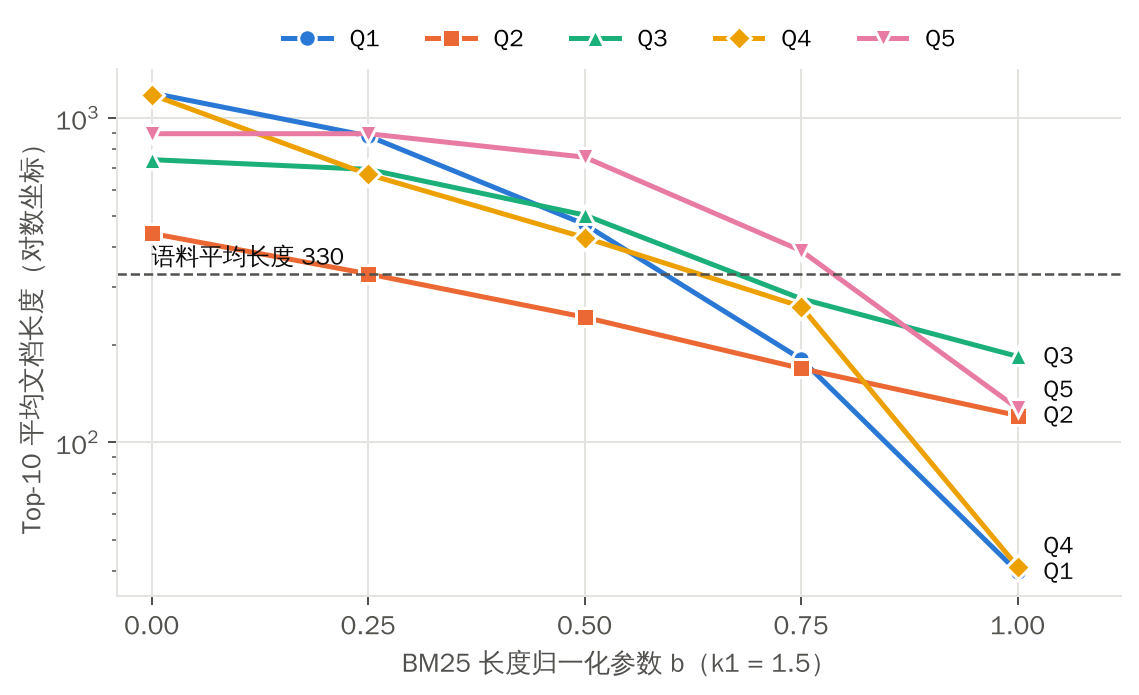
\includegraphics[width=0.88\textwidth]{figures/fig_b_sweep.png}
\caption{BM25 参数 $b$ 对 Top-10 平均文档长度的影响}
\label{fig:bsweep}
\end{figure}

\begin{table}[H]
\centering
\caption{不同 $b$ 取值下 Top-10 的平均文档长度（词项数）}
\label{tab:bsweep}
\begin{tabular}{@{}lrrrrr@{}}
\toprule
$b$ & Q1 & Q2 & Q3 & Q4 & Q5 \\
\midrule
0.00 & 1193.0 & 440.5 & 743.3 & 1178.8 & 893.5 \\
0.25 & 879.5 & 330.5 & 693.8 & 669.4 & 893.5 \\
0.50 & 469.9 & 243.0 & 501.7 & 427.5 & 756.6 \\
0.75 & 180.5 & 168.9 & 277.1 & 262.1 & 389.6 \\
1.00 & 39.9 & 120.9 & 184.0 & 41.4 & 127.3 \\
\bottomrule
\end{tabular}
\end{table}

随着 $b$ 从 0 增大到 1，五条查询 Top-10 的平均长度都单调下降，跨度达到一个数量级。$b = 0$ 时 BM25 完全不考虑文档长度，Top-10 被上千词项的长文占据；$b = 1$ 时，Q1 和 Q4 的 Top-10 平均长度降到约 40 个词项，已经接近 TF-IDF 的水平。我们采用的 $b = 0.75$ 使五条查询的 Top-10 平均长度落在 169 至 390 之间，正好处于语料平均长度附近。

\subsection{预处理与查询设计的对照实验}
\label{sec:ablation}

\textbf{词干还原。} 表~\ref{tab:stem} 比较了启用与不启用词干还原时，BM25 对五条查询的命中文档数，以及两种设置下 Top-10 的重合篇数。

\begin{table}[H]
\centering
\caption{词干还原对 BM25 检索的影响}
\label{tab:stem}
\resizebox{\textwidth}{!}{\begin{tabular}{@{}lllrrr@{}}
\toprule
查询 & 被归并的主要变形（不还原时的文档频率） & 还原后词项（文档频率） & 命中（还原） & 命中（不还原） & Top-10 重合 \\
\midrule
Q1 & hurricane 621，hurricanes 106 & hurrican 672 & 672 & 621 & 6 \\
Q2 & george 1,225，georges 123 & georg 1,353 & 1,861 & 1,752 & 3 \\
Q3 & bill 2,348，bills 567，billed 85 & bill 2,849 & 7,474 & 7,043 & 9 \\
Q4 & down 6,830，downs 111，downed 70 & down 6,941 & 7,212 & 7,102 & 10 \\
Q5 & strike 1,097，strikes 1,275 & strike 2,345 & 2,716 & 1,418 & 7 \\
\bottomrule
\end{tabular}}
\end{table}

词干还原使五条查询的命中数都有所增加，其中 Q5 的命中数几乎翻倍，因为“strikes”的文档频率甚至高于“strike”。对 Top-10 影响最大的是 Q2：不做词干还原时，“george”无法匹配“georges”，Top-10 中只有 3 篇与默认配置相同，而且没有一篇含有“georges”。这十篇文档中有 5 篇是因为 NBC 记者 George Lewis 的署名而命中 \texttt{george}，2 篇提到的是前总统 George Bush，只有 1 篇是把飓风名拼写为“Hurricane George”的 VOA 报道。

\textbf{短语的软匹配与硬匹配。} 在 Q4 上，硬匹配只保留含有完整短语的 406 篇文档，软匹配则对 7,212 篇文档打分。尽管候选集合相差十余倍，两种方式给出的 Top-10 却完全相同，BM25 和 TF-IDF 都是如此，因为软匹配下 Top-10 的十篇文档本来就全部包含该短语。此外，全语料中同时含有 \texttt{newt} 和 \texttt{gingrich} 的文档共 409 篇，其中只有 3 篇二者不相邻。

\textbf{连字符词的匹配方式。} 表~\ref{tab:hyphen} 比较了 Q5 中 \texttt{closed-door} 的三种处理规则。

\begin{table}[H]
\centering
\caption{Q5 中连字符词的三种处理规则（Top-10 中的文档数）}
\label{tab:hyphen}
\resizebox{\textwidth}{!}{\begin{tabular}{@{}llrr@{}}
\toprule
打分函数 & 连字符词规则 & 含 nba 的文档 & 含短语 closed door 的文档 \\
\midrule
\multirow{3}{*}{BM25} & 短语 + 组成词（与引号短语相同） & 1 & 9 \\
& 仅短语（默认） & 8 & 3 \\
& 仅组成词 & 8 & 2 \\
\midrule
\multirow{3}{*}{TF-IDF} & 短语 + 组成词（与引号短语相同） & 4 & 6 \\
& 仅短语（默认） & 10 & 0 \\
& 仅组成词 & 10 & 0 \\
\bottomrule
\end{tabular}}
\end{table}

在 BM25 下，把连字符词同时展开为短语和组成词时，Top-10 中只有 1 篇与 NBA 有关，而含有“closed door”的文档占了 9 篇；改为只构成一个短语单元后，NBA 相关文档增至 8 篇，同时仍有 3 篇含有“closed door”，包括那篇唯一同时命中三个查询单元的 NYT 报道。只拆成独立组成词时，NBA 相关文档同样为 8 篇，含有“closed door”的文档降为 2 篇。这一规则排在第 1 名的是一篇高度相关的 CNN 报道，原文为“NBA owners and players have closed the door to the media by conducting secret meetings”，其中“closed”与“door”之间隔着“the”，在仅短语规则下这篇文档只排在第 119 名。但同一规则下的第 2、4、7、10 名之所以得分，是因为词干还原后的 \texttt{close} 匹配了“close to \$900 million”“come close”“more closely”等与闭门会议无关的用法。

\section{结果分析}

\subsection{TF-IDF 的余弦归一化偏向极短文档}

TF-IDF 结果中短文档的集中，可以从公式~\eqref{eq:tfidf} 直接推出。对单词查询而言，查询向量归一化后权重为 1，文档得分退化为 $(1 + \log_{10}\mathrm{tf}_{u,d}) / \lVert d \rVert$。分子随词频只按对数增长，分母 $\lVert d \rVert$ 却大致随文档中不同词项的数量按平方根增长。以 Q1 为例，冰球预告只有 13 个词项，$\lVert d \rVert = 3.52$，“hurricanes”只出现一次，得分为 $1 / 3.52 = 0.2841$；BM25 排名第 4 的 VOA 飓风报道长 577 个词项，“hurricane”出现了 16 次，分子为 $1 + \log_{10}16 = 2.20$，但 $\lVert d \rVert = 19.54$，得分只有 0.1128。文档中十几次的重复提及抵不过分母的增长，于是只要某个查询词在一句简短的串场词里出现一次，这篇文档就能排到所有完整报道之前。

TDT3 的构成把这种偏向放大到了极端。语料中有 11,954 个 CNN 片段，长度中位数只有 63 个词项，其中大量是“下节预告”式的一句话。它们为热门话题提供了一批“全文不超过 30 个词项、却含有查询词”的候选文档：含 \texttt{hurricane} 的有 40 篇，含 \texttt{nba} 的有 18 篇，含短语“newt gingrich”的有 10 篇。这样的候选数量已经足以填满 Top-10，TF-IDF 的 Top-10 因此几乎被 CNN 包揽：Q4 为 10 篇，Q5 为 9 篇。多词查询的情况更不利。余弦得分是各单元贡献之和，而一篇十几个词的短文档通常只容得下一两个查询词，于是 Q2 至 Q5 的 TF-IDF Top-10 中，包含全部查询单元的文档只有 3、3、0、0 篇。BM25 在这几条查询上分别为 10、10、9、1 篇，Q5 的 1 篇也已达到语料所能提供的上限。

这些短文档并非全都与查询无关。TF-IDF 对 Q5 返回的十篇简讯全部涉及 NBA 停摆，主题判断是正确的。问题在于它们的信息量很少，而且没有覆盖查询中的“strike”和“closed-door”两个限定条件。对用户而言，BM25 返回的完整报道更有用。

\subsection{BM25 的长度归一化与词频饱和}

BM25 能避免上述偏向，靠的是两个与 TF-IDF 不同的机制。第一，词频饱和：公式~\eqref{eq:bm25} 中的分式随 $\mathrm{tf}_{u,d}$ 增长并趋于 $k_1 + 1$，一个查询词的贡献只取决于它自身的词频和文档长度，而在 lnc 方案中，文档里其他所有词项都会通过 $\lVert d \rVert$ 稀释查询词的权重。第二，长度归一化：BM25 的长度惩罚是相对于 $\mathrm{avgdl}$ 的线性插值，强度由参数 $b$ 控制，而余弦归一化把每篇文档硬性缩放到单位长度，没有可以调节的余地。

$b$ 值实验验证了第二个机制是长度特征的主要来源。$b = 0$ 时长文因词频高而占优，Top-10 平均长度在 440 到 1,193 个词项之间；$b = 1$ 时长度惩罚完全按比例施加，Q1 和 Q4 的 Top-10 退化为约 40 个词项的短片段，表现出与 TF-IDF 相似的偏向。$b = 0.75$ 在两者之间取得了平衡，Top-10 平均长度贴近语料平均值。由此可见，BM25 与 TF-IDF 在本实验中的差别，主要来自对文档长度的处理方式，而不是对词项权重的定义。

单词查询 Q1 的得分分布还反映了词频饱和的效果。十篇结果的得分都在上限 10.06 的 86\% 至 88\% 之间，彼此只差 0.21。全语料中“hurricane”出现次数最多的是一篇 NYT 长文，出现了 22 次，但它长达 2,330 个词项，BM25 得分只有 7.30，没有进入 Top-10。高词频带来的增益已经饱和，抵不过长度带来的惩罚。

\subsection{词干还原的两面作用}

词干还原对五条查询的影响方向并不一致。Q2 是收益最明显的例子。“george”与“georges”被归并为同一词项，原本只代表人名的查询因此覆盖了飓风 Georges：启用词干还原时，Top-10 的十篇文档都同时含有两个查询词，且都是关于飓风的报道；不做词干还原时，Top-10 有一半是靠 NBC 记者 George Lewis 的署名才命中的。需要指出的是，这一收益带有偶然性：Porter 算法删去的是英语复数词尾“s”，它恰好与这个法语名字的拼写重合，我们的预处理并不理解“Georges”是一个飓风的名字。

同一机制在 Q3 上带来了错误匹配。“billed”被还原为 \texttt{bill}，使 CNN 的一篇谈判报道因为“being billed”一词进入了 BM25 的 Top-10。在 Q1 上，TF-IDF 排名第 1 的冰球队“Hurricanes”也是借助词干还原才与“hurricane”匹配上的。词干还原和小写化合在一起，抹去了“Bill/bill”“Hurricanes/hurricanes”之间原本可以靠大小写和单复数区分的专名信息。

综合来看，词干还原在本实验中的总体作用偏正面：它提高了五条查询的召回，其中 Q5 的命中数几乎翻倍；它引入的错误匹配主要出现在专名与普通词同形的场合。在多词查询中，这类错误匹配对排序的影响较为有限，因为一篇文档要排进前列，还需要同时命中其他查询词。Q3 的“Bill Hazard”一文正是如此：它的“Bill”是记者署名，但这篇文档同时含有 \texttt{clinton} 和 \texttt{israel}，主体也确实是克林顿出访前的以色列局势，所以错误匹配并没有把无关文档推到前列。

\subsection{短语与连字符的设计取舍}

软匹配与硬匹配在 Q4 上给出完全相同的 Top-10，这说明对于“newt gingrich”这样高度专指的短语，软匹配并不会让不含短语的文档挤进前列。原因有两层。其一，含有短语的文档比只零散含有组成词的文档多出一份短语单元的得分，而这个单元的逆文档频率很高（406 篇文档，BM25 逆文档频率为 4.53）。其二，在这个语料中，“newt”和“gingrich”几乎总是相邻出现：同时含有二者的 409 篇文档中只有 3 篇不相邻，所以软匹配额外纳入的候选文档大多只含其中一个词，或者只含 \texttt{down}，它们本来就无法与含有完整短语的文档竞争。软匹配真正发挥作用的场合，是短语在语料中很少出现、甚至不出现的时候：这时硬匹配会直接返回空结果，而软匹配仍能按组成词给出排序。在作业提供的这条测试查询上，两种方式没有区别，但软匹配在更多情形下能返回有用的结果。

连字符实验则说明，查询单元的个数本身就是一种隐性权重。“短语加组成词”的规则对引号短语是合理的，因为用户用引号明确表达了“这几个词作为一个整体很重要”。但如果对连字符词套用同一规则，一个本来只是普通复合词的查询词就会获得三倍权重，Q5 的 Top-10 因而被“closed-door talks”这类与 NBA 无关的报道占据。改为“一个连字符词只构成一个短语单元”之后，每个查询词在单元数上重新变得平等，排序回到以 \texttt{nba} 这个最具区分度的词为主导。“只拆成独立组成词”的规则同样使各查询词的单元数平等，并且因为不要求词序，它找到了一篇改写为“closed the door”的相关报道，这是仅短语规则做不到的。但放弃词序约束的代价同样明显：在词干还原的作用下，\texttt{close} 会匹配“close to”“closely”等意义完全不同的用法，Top-10 中有四篇文档就是这样获得了得分。两种规则在 NBA 相关文档数上打成平手，区别在于各自引入的误差：仅短语规则会漏掉词序被改写的表达，仅组成词规则则会混入大量与“闭门”无关的匹配。考虑到连字符复合词在英语中通常作为固定搭配出现，我们选择以词序约束换取匹配精度，把仅短语规则作为默认设置，同时保留 \texttt{--hyphen=parts} 选项供需要更高召回时使用。

\subsection{系统效率}

索引构建只需约 22 秒，查询延迟在 14 毫秒以内，这主要得益于两个设计。其一，倒排表采用紧凑的整数数组，加载时反序列化的对象数量少，索引加载只需约半秒；其二，打分按单元顺序累加，每个单元只遍历一次自己的倒排表，代价与查询词的文档频率之和成正比。Q3 和 Q4 含有 \texttt{clinton}、\texttt{down} 这样文档频率在 4,000 以上的词，因此打分耗时比只含低频词的 Q1 多出一个数量级，但仍在 3 毫秒以内。短语求交需要先展开各词的位置表，这部分开销集中在含短语的 Q4 和 Q5 上，在当前规模下同样可以忽略。真正占用时间的是摘要生成，它需要从磁盘读取十篇原文并逐窗口扫描，占据了一次查询的大部分耗时。

\section{结论}

我们用 Python 从零实现了一个面向 TDT3 语料的命令行搜索引擎。系统包含自行实现的 Porter 词干算法、对数字缩写与连字符作针对性处理的分析器、基于紧凑整数数组的位置倒排索引、支持引号短语软匹配的查询解析器、BM25 与 TF-IDF 两种手写打分函数，以及查询相关摘要生成。37,526 篇文档的索引在约 22 秒内建成，五条测试查询的延迟都在 14 毫秒以内，返回条数可以通过 \texttt{--hits} 选项配置，每条结果依次给出排名、得分、文档编号和查询相关摘要。我们实现的 Porter 算法在 110,617 个词上与 NLTK 的原论文模式逐一比对，仅在 27 个两字母词上因长度约定不同而有差异。

在五条测试查询上，BM25 返回的 Top-10 在主题上都与查询相符，并且在多词查询上覆盖了尽可能多的查询单元。TF-IDF 的 lnc.ltc 方案则表现出强烈的短文档偏向：它的 Top-10 平均长度只有 18 至 64 个词项，多由一两句话的广播串场词组成。BM25 的参数实验表明，二者差异的根源在于长度归一化方式。余弦归一化让 TDT3 中数量庞大的 CNN 短片段获得了不成比例的优势，而 BM25 的 $b = 0.75$ 使结果长度贴近语料平均水平。

对照实验也为几项预处理与查询设计提供了依据。词干还原提高了全部五条查询的召回，并借“georges”的归并显著改善了 Q2，代价是在 Q3 等查询上引入了专名与普通词混同的错误匹配。不删除停用词保留了 Q4 中关键的 \texttt{down}，而它的权重已由逆文档频率适度压低。引号短语的软匹配在 Q4 上与硬匹配结果一致，在短语稀少的场合则能避免返回空结果。对连字符词，我们发现查询单元的个数本身就是一种隐性权重。把一个连字符词只当作一个短语单元，能在保留词序信息的同时使各查询词的权重保持均衡，Q5 的 Top-10 中 NBA 相关报道因此从 1 篇增加到 8 篇；它的代价是会漏掉“closed the door”这类改写了词序的表达。

\appendix

\section{TF-IDF（lnc.ltc）的 Top-10 结果截图}
\label{app:tfidf}

图~\ref{fig:t1} 至图~\ref{fig:t5} 是以 \texttt{--model=tfidf} 选项执行五条测试查询时的控制台输出，其余设置与正文中的 BM25 结果相同。

\begin{figure}[H]
\centering
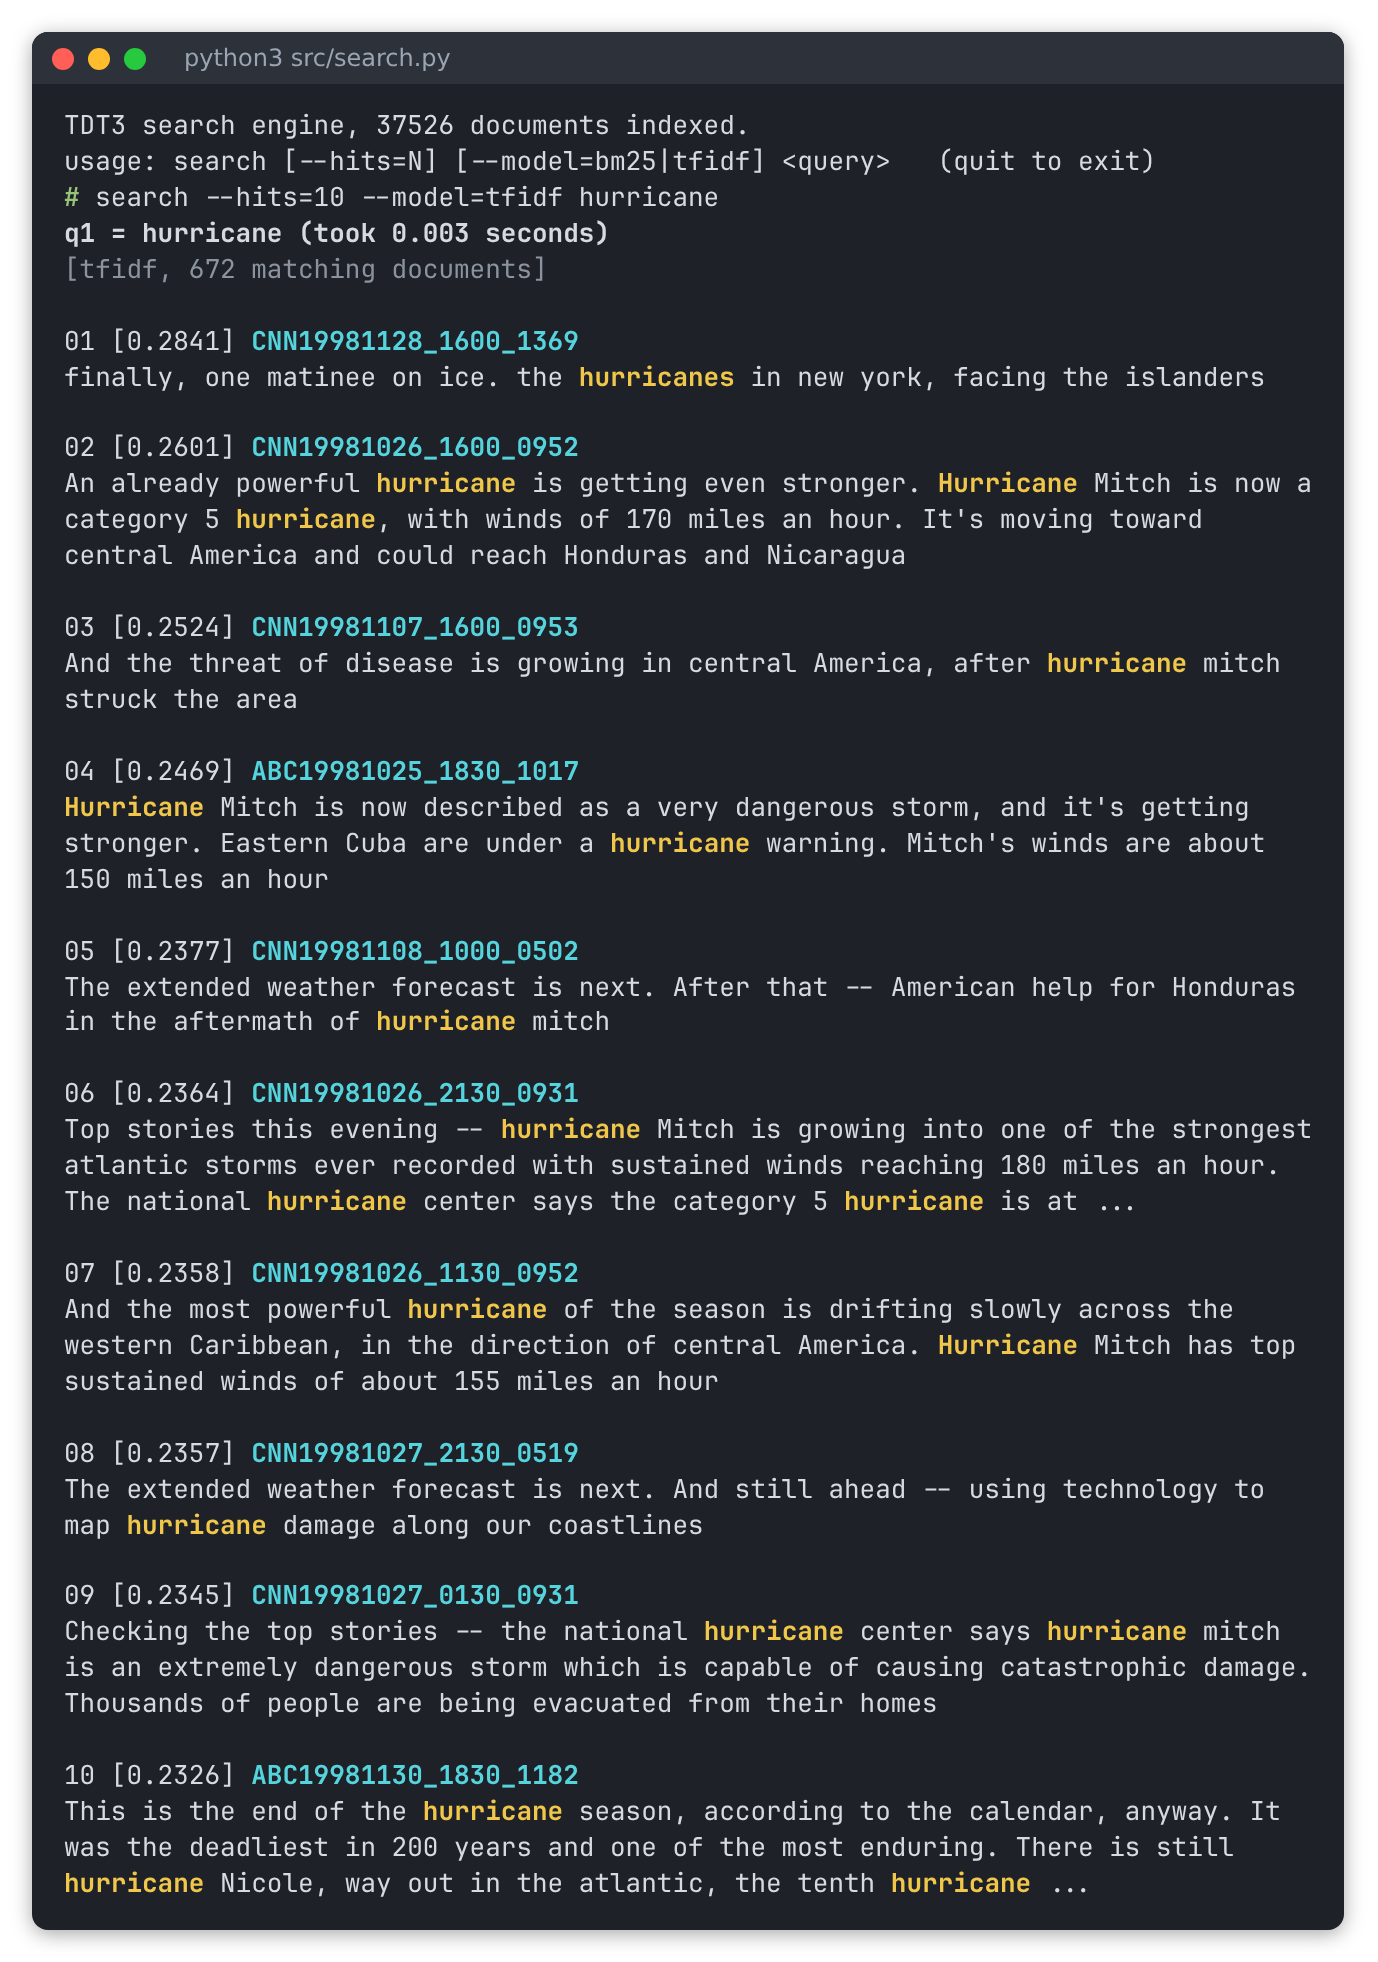
\includegraphics[width=0.78\textwidth]{figures/screen_q1_tfidf.png}
\caption{Q1 \texttt{hurricane} 的 TF-IDF Top-10 结果}
\label{fig:t1}
\end{figure}

\begin{figure}[H]
\centering
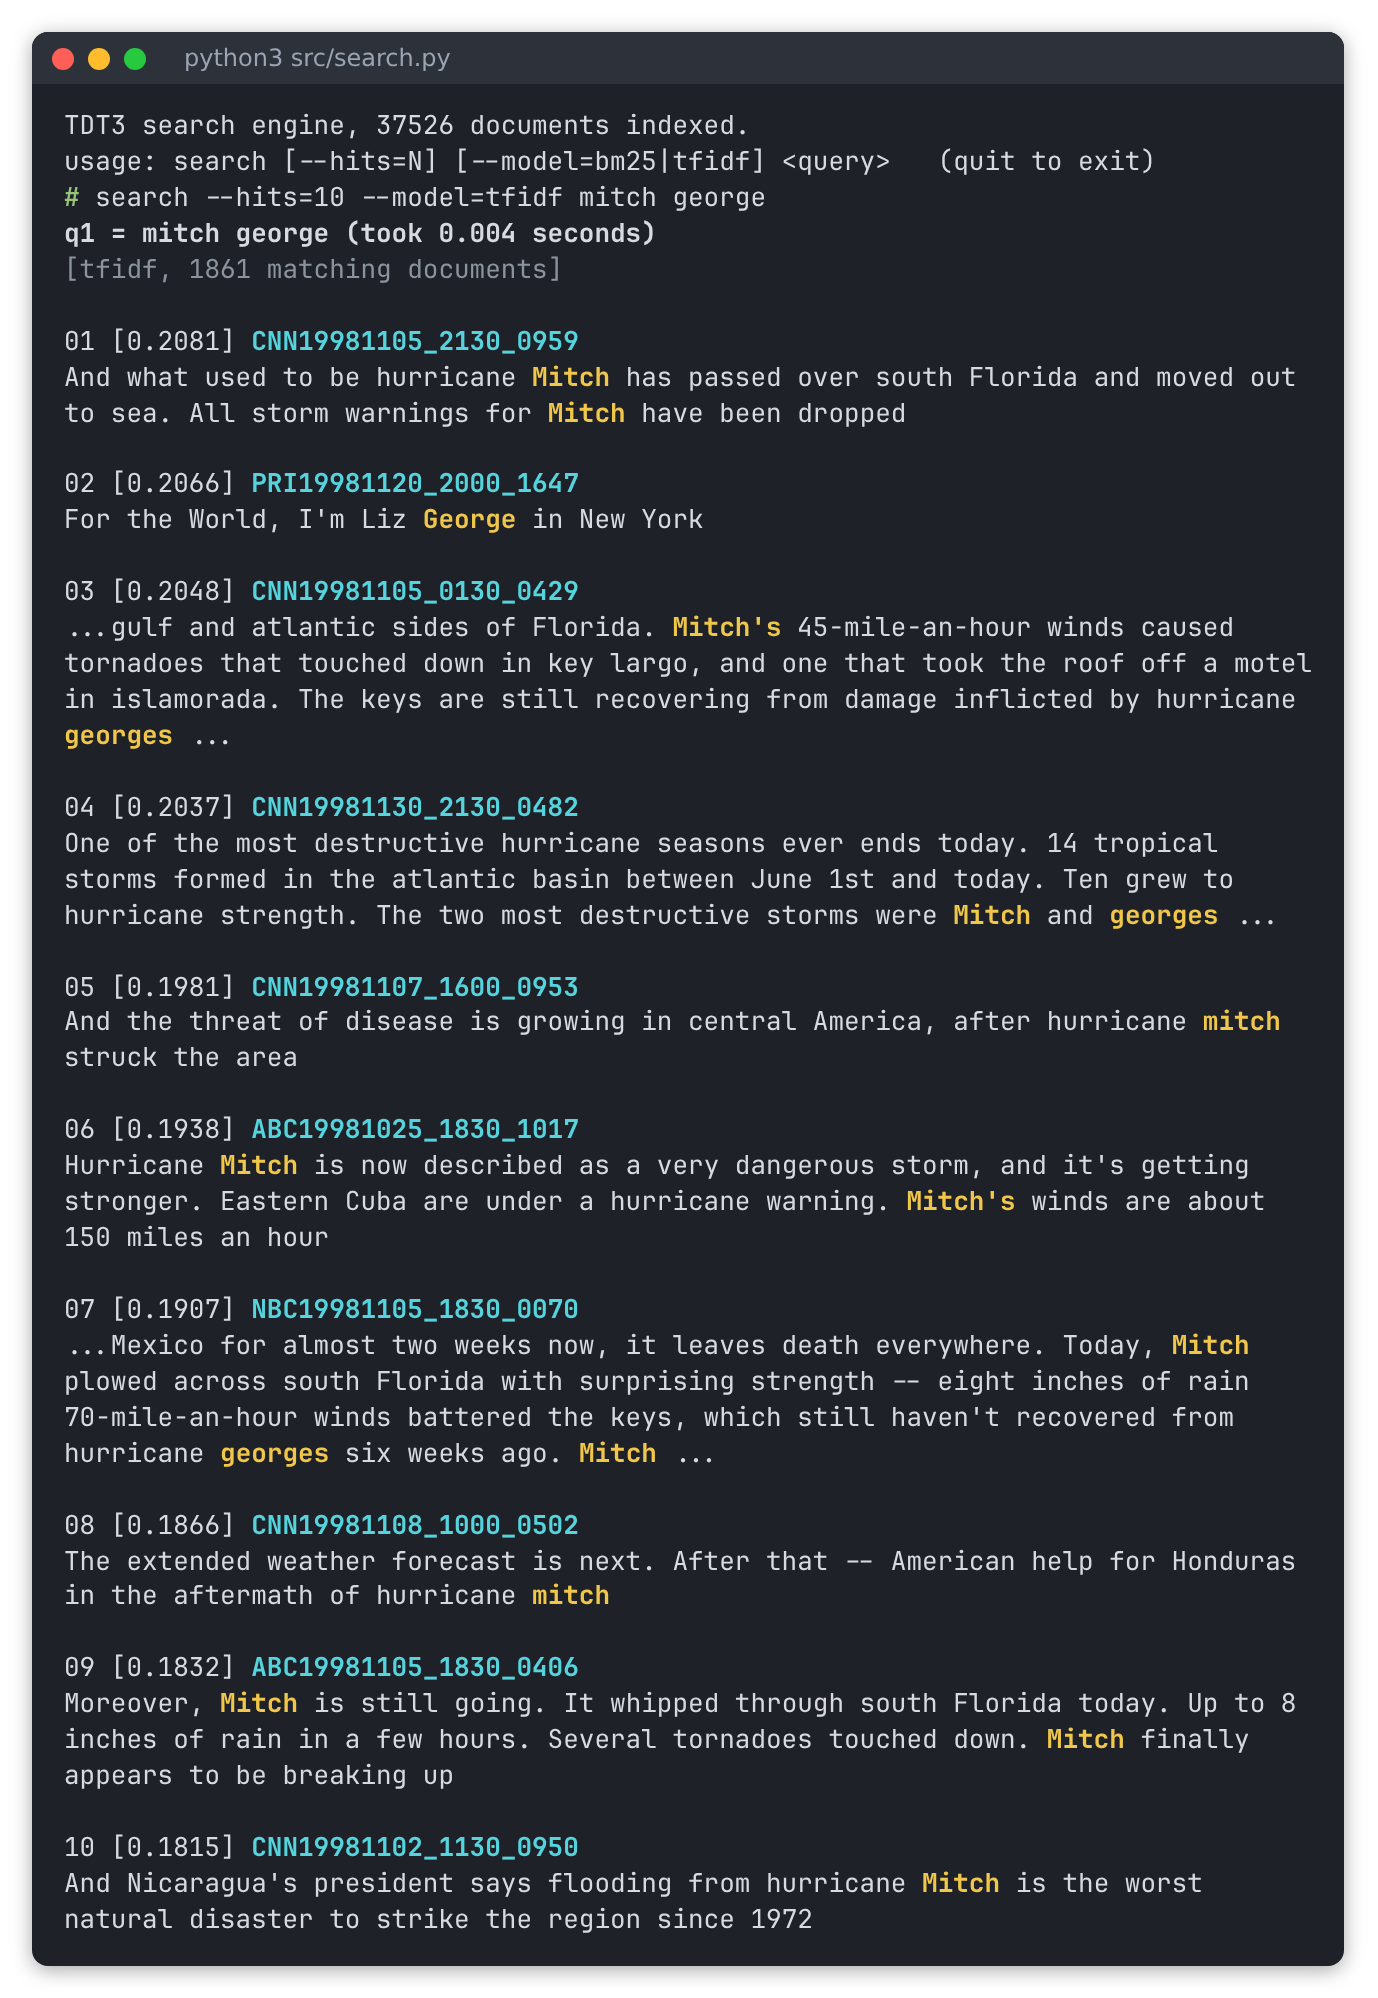
\includegraphics[width=0.78\textwidth]{figures/screen_q2_tfidf.png}
\caption{Q2 \texttt{mitch george} 的 TF-IDF Top-10 结果}
\label{fig:t2}
\end{figure}

\begin{figure}[H]
\centering
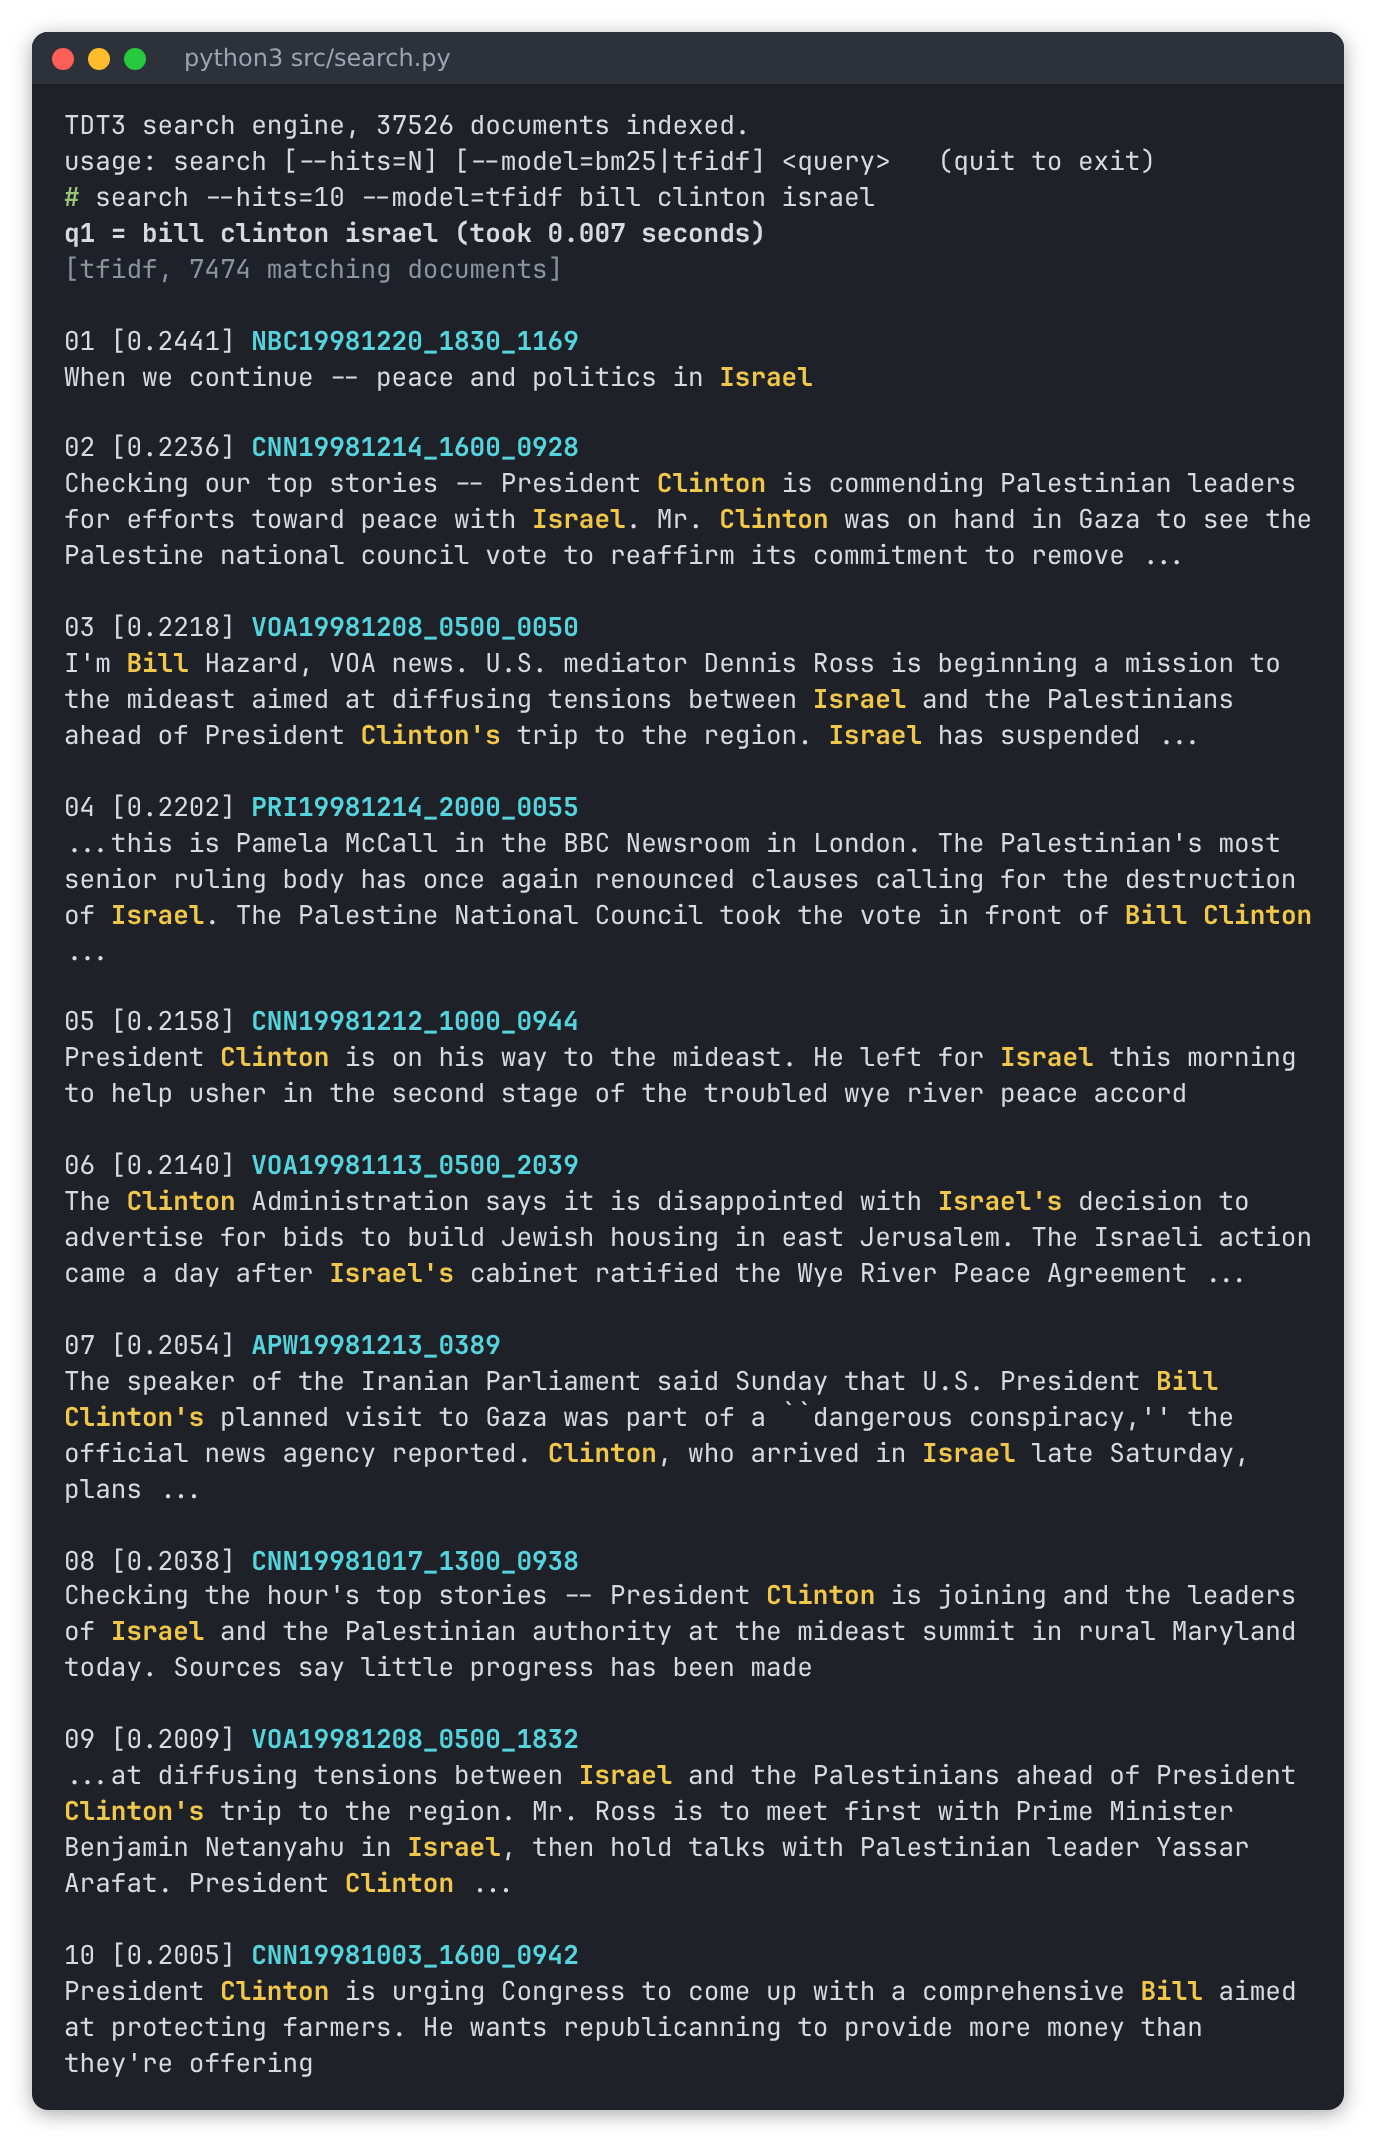
\includegraphics[width=0.78\textwidth]{figures/screen_q3_tfidf.png}
\caption{Q3 \texttt{bill clinton israel} 的 TF-IDF Top-10 结果}
\label{fig:t3}
\end{figure}

\begin{figure}[H]
\centering
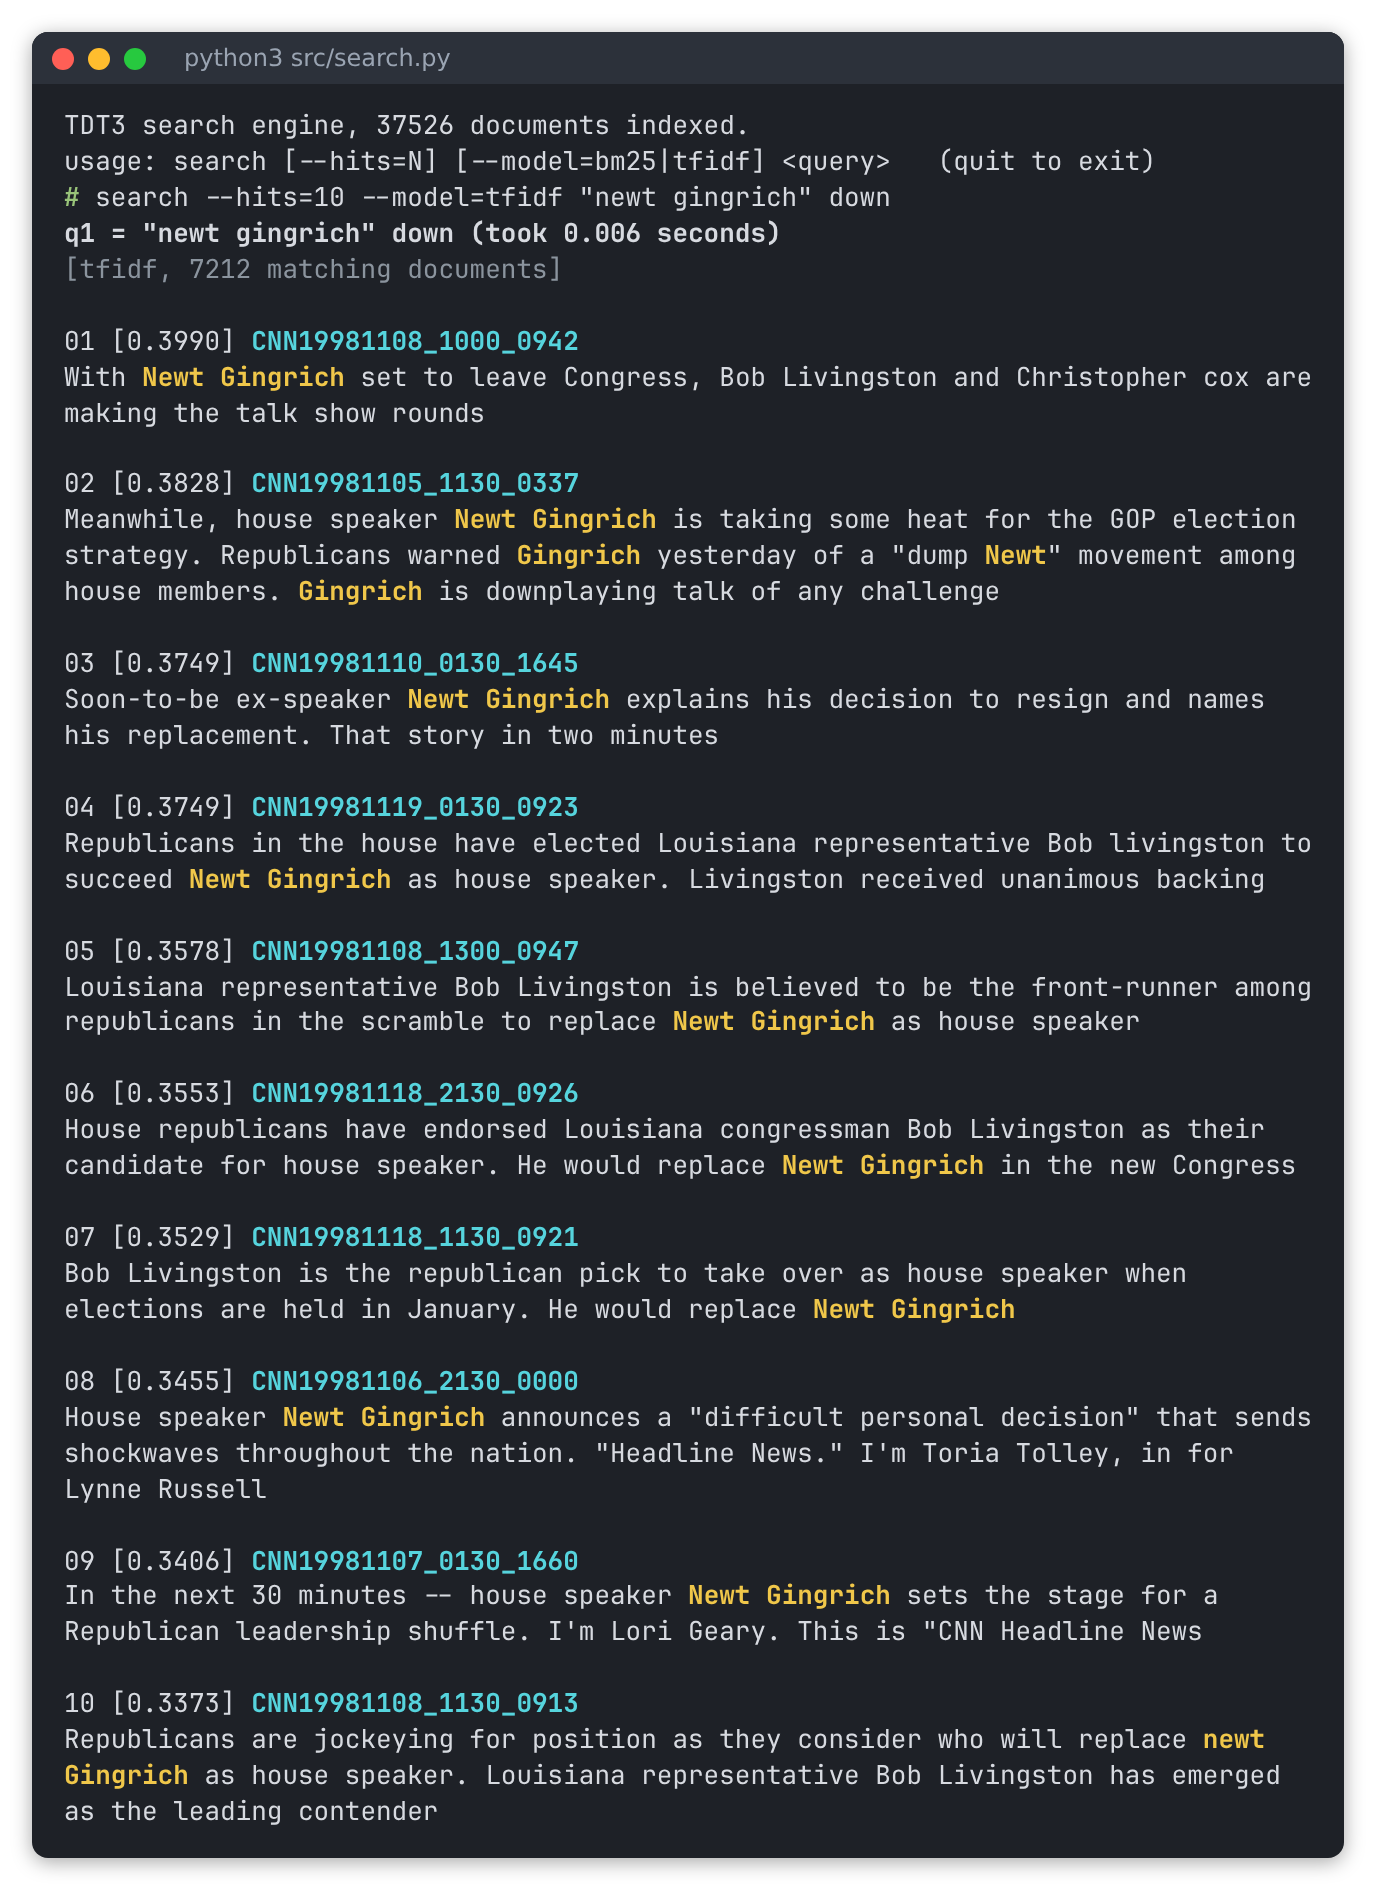
\includegraphics[width=0.78\textwidth]{figures/screen_q4_tfidf.png}
\caption{Q4 \texttt{"newt gingrich" down} 的 TF-IDF Top-10 结果}
\label{fig:t4}
\end{figure}

\begin{figure}[H]
\centering
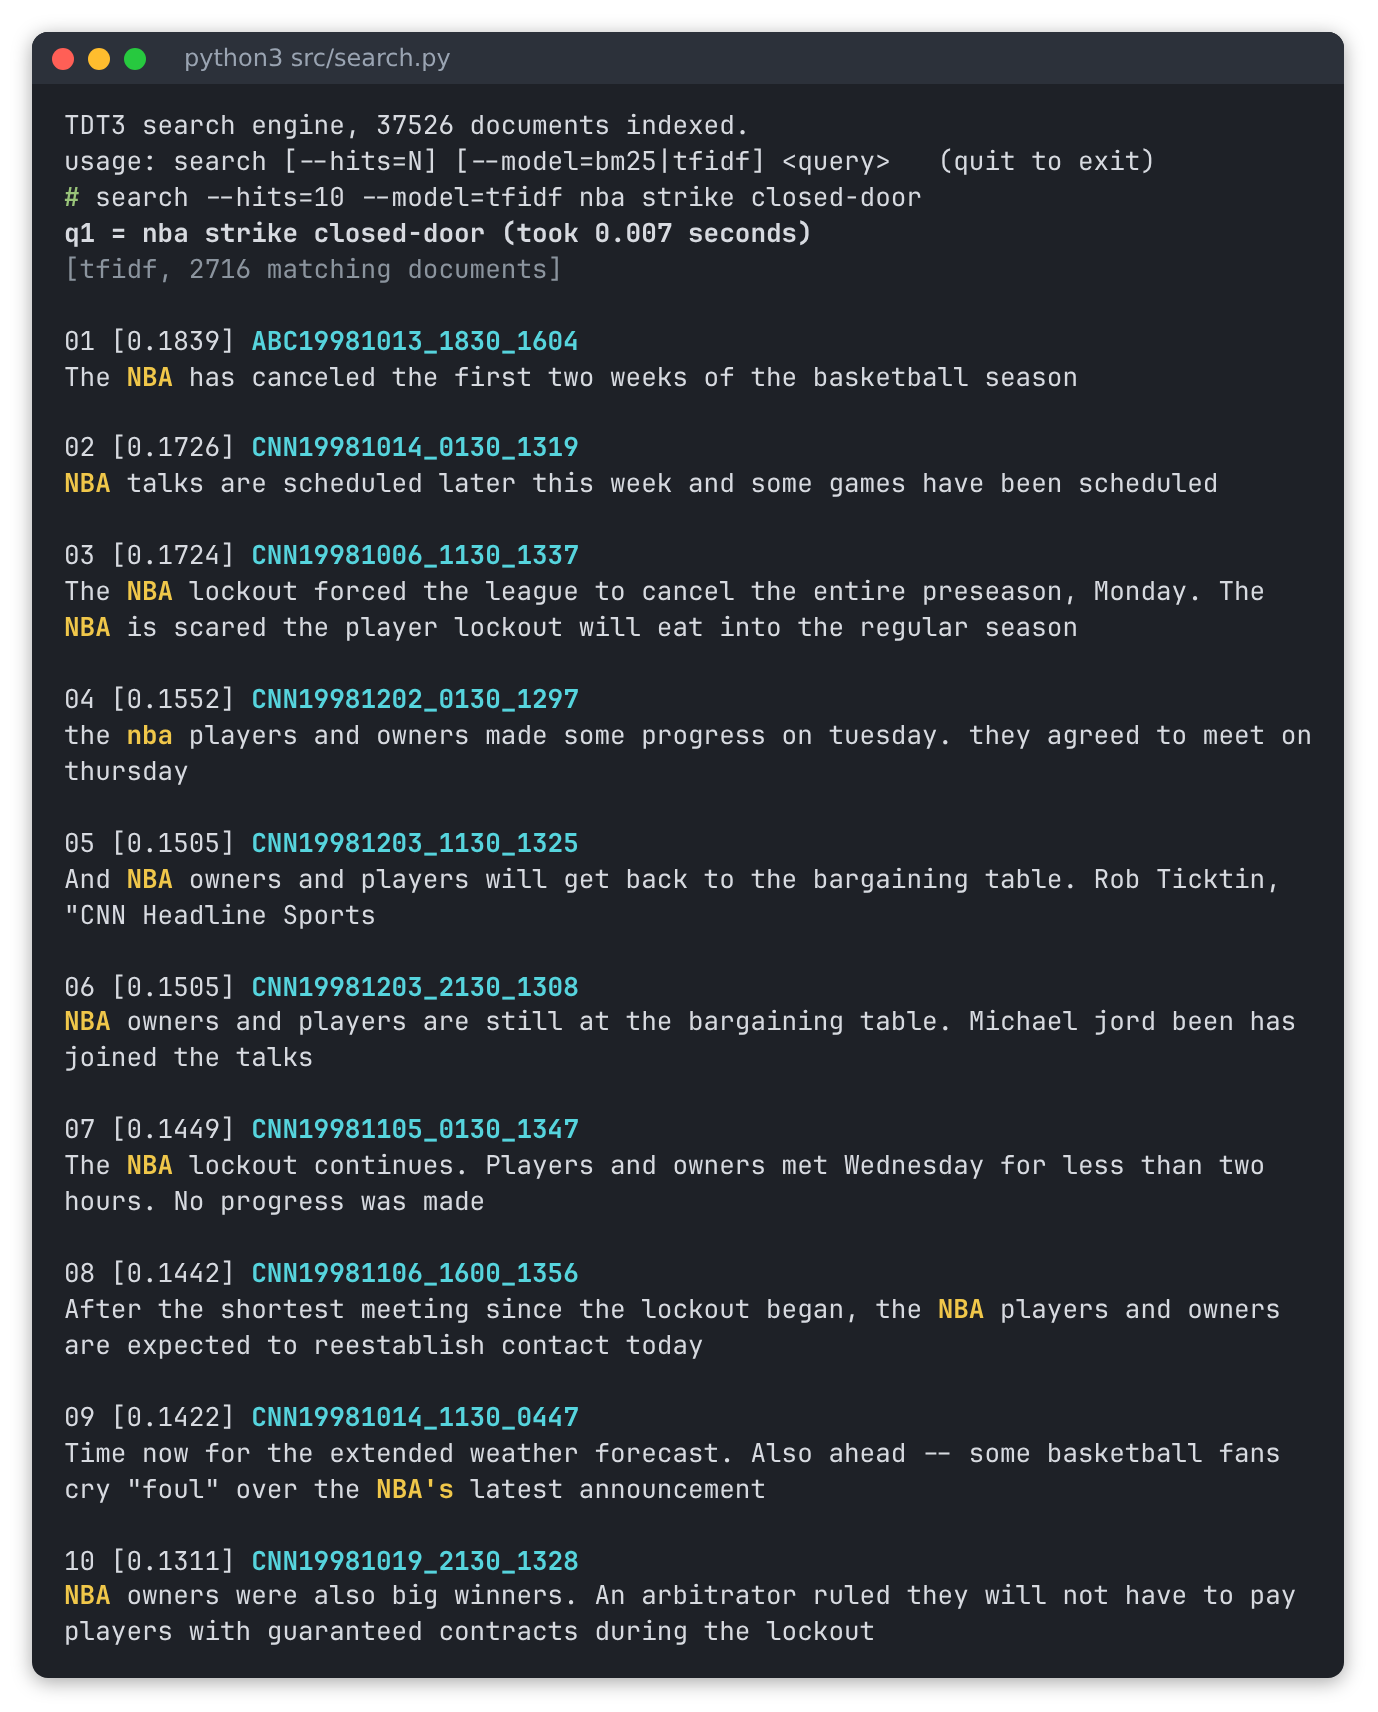
\includegraphics[width=0.78\textwidth]{figures/screen_q5_tfidf.png}
\caption{Q5 \texttt{nba strike closed-door} 的 TF-IDF Top-10 结果}
\label{fig:t5}
\end{figure}

\end{document}
